The once-through transition scenarios are compared on multiple 
criteria: the energy supplied by the reactors, the number of advanced reactors deployed, 
the uranium resources required, the amount of \gls{SWU} capacity required 
to enrich uranium,
and the mass of waste produced. Each of these metrics can be used to inform 
policies and decisions of potential deployment schedules and the 
fuel cycle infrastructure required to support the deployment schedule. 

Bachmann et al. \cite{bachmann_enrichment_2021} presents a subset of 
these results for similar scenario definitions, except in that work 
they assumed the 
\glspl{LWR} operate for 60 years if they are not closed before December 
2020. This difference in 
the assumed lifetime of the \glspl{LWR} impacts the energy demand, 
the deployment schedule of advanced reactors, and the material 
requirements of the advanced reactors because a different number of 
\glspl{LWR} are operating when the transition begins. The results of 
Scenario 1 (only \glspl{LWR} with no transition to advanced reactors) 
are presented first. Then, each result for the transition scenarios are 
presented, first for the the no growth scenarios 
(Scenarios 2-7) then for the 1\% growth scenarios (Scenarios 
8-13).

\section{Scenario 1: LWRs only}\label{sec:scenario1}
Scenario 1 models only the \glspl{LWR} deployed in the United States with no 
prescribed energy demand. This scenario provides insight on historical 
requirements of the nuclear industry as well as future demands if the 
US does not deploy any new reactors and decommissions current reactors at 
their current license expiration. The 
deployment and material requirements of the \glspl{LWR} will be the same 
for each of the other scenarios (Scenarios 2-13). Therefore analysis 
of the other scenarios will focus on the requirements of 
the advanced reactors deployed. Therefore, the results of Scenarios 2-13 
can be compared with the results of Scenario 1 to provide a comparison 
of material requirements between new and current reactors. 

Figure \ref{fig:energy_reactor1} shows the number of 
reactors deployed in Scenario 1 as a function of time and the energy 
produced by the \glspl{LWR} each year. The energy produced by the 
\glspl{LWR} scales with the number of reactors deployed, as 
one would expect. This scenario deploys a maximum of 109 
\glspl{LWR} at one time, producing 
between \hl{101.24-102.46} GWe-yr, and deploys 92 \glspl{LWR}
when the transition begins in January 2025. The first \gls{LWR} is 
commissioned in August 1967, and all of the \glspl{LWR} are
decommissioned by October 2055. In 2025, the \glspl{LWR} produce 
89.456 GWe-y of energy, which is the basis of the energy demand for 
the other scenarios. 

\begin{figure}
    \centering
    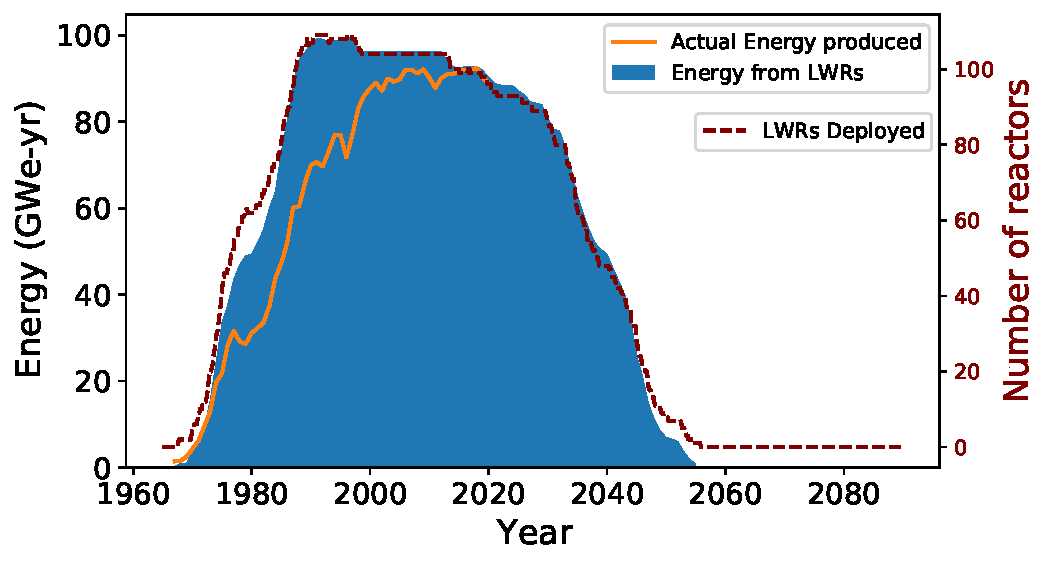
\includegraphics[scale=0.8]{s1_energy_reactors.pdf}
    \caption{Energy supplied by \glspl{LWR} in Scenario 1 during each year of
    the simulation compared to the number of reactors deployed.}
    \label{fig:energy_reactor1}
\end{figure}

Figure \ref{fig:energy_reactor1} also \hl{shows actual historic data} of the 
energy generated by nuclear reactors in the US \cite{noauthor_total_2022}.
 However 
the \gls{LWR} fleet has operated at a variety of capacity factors, often 
lower than 94\%. The lower capacity factor results from outages that last 
longer than 1 month and unplanned outages. The difference 
in the simulated and historic energy production suggests that the modeled 
energy production in 2025 is probably higher than what will actually 
be produced. Therefore, the transitions in this work will model an upper 
bound of resources required to meet the needs of each transition. 

The mass of enriched uranium sent to the \glspl{LWR} in this scenario (Figure 
\ref{fig:fuel1}) follows the general pattern of the reactor deployment, but with 
more variation between individual time steps. The increased variation between 
time steps is because of the staggering of outages for the reactors, or when 
they receive fuel. Times that receive more fuel correspond with more 
\glspl{LWR} undergoing refueling outages. There are also times with large 
increases in the mass of fuel 
sent to the reactors, such as in 2016, because these times include the deployment 
of a new reactor with a full core of fuel instead of the smaller amount 
required for refueling.

The maximum amount of enriched uranium sent to the \glspl{LWR} at any one 
time in this scenario is 513.72 MTU, which occurs in the 1980s. The 
average mass of enriched uranium sent to 
the reactors for the entire scenario is 135.74 MTU/month. The average mass of 
enriched uranium sent to the \glspl{LWR} between when they are first deployed 
and 2025 is 164.92 MTU/month. This average is larger than what is reported in 
\cite{bachmann_enrichment_2021} because the average reported by 
Bachmann et al. accounts for the time before the \glspl{LWR} are  
deployed while the average reported here does not. The average mass of 
uranium sent to \glspl{LWR} between 2025-2055, from the start of the transition 
to when they are all decommissioned is 81.11 MTU/month. Comparing the averages 
shows that the vast majority of enriched uranium is sent to the \glspl{LWR} 
before 2025, which matches with the decline in the number of \glspl{LWR} 
deployed after 2020. After 2025, a cumulative total of 29,848.6 MTU is 
sent to the \glspl{LWR},
which is less than the cumulative mass reported in \cite{bachmann_enrichment_2021}
because Bachmann et al. assumed that all \glspl{LWR} would operate for 60 years, 
which is longer than the assumed operating time for some \glspl{LWR} in 
this work. This scenario requires a total of 143,479 MT of enriched uranium.

\begin{figure}
    \centering
    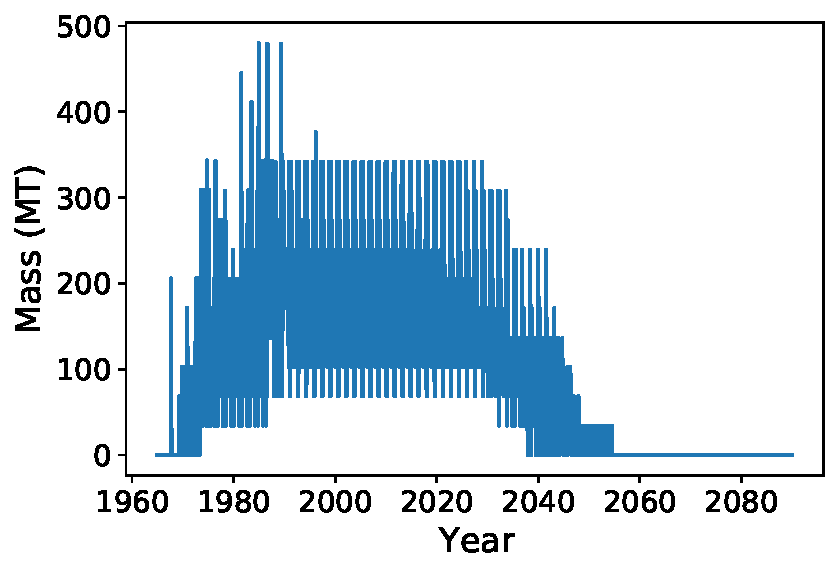
\includegraphics[scale=0.8]{s1_uox.pdf}
    \caption{Mass of uranium supplied to the LWRs in Scenario 1 at each time step.}
    \label{fig:fuel1}
\end{figure}

The next metric of interest for this work is the mass of natural uranium 
required as feed material to produce the enriched uranium for the 
reactors, shown in Figure \ref{fig:feed1}. The mass of feed uranium 
is about an order of magnitude larger than the mass of the enriched uranium. 
Scenario 1 requires a maximum of 4,121.8 MT of 
feed uranium at one time and an average of 1,089.1 MT/month of natural uranium 
when \glspl{LWR} are deployed. Before 2025, this scenario requires an average of 
1,323.2 MTU/month of natural uranium, and requires an average of 650.8 MTU/month 
after 2025. In total, the \glspl{LWR} require 1,151,208 MT of feed uranium.

\begin{figure}
    \centering
    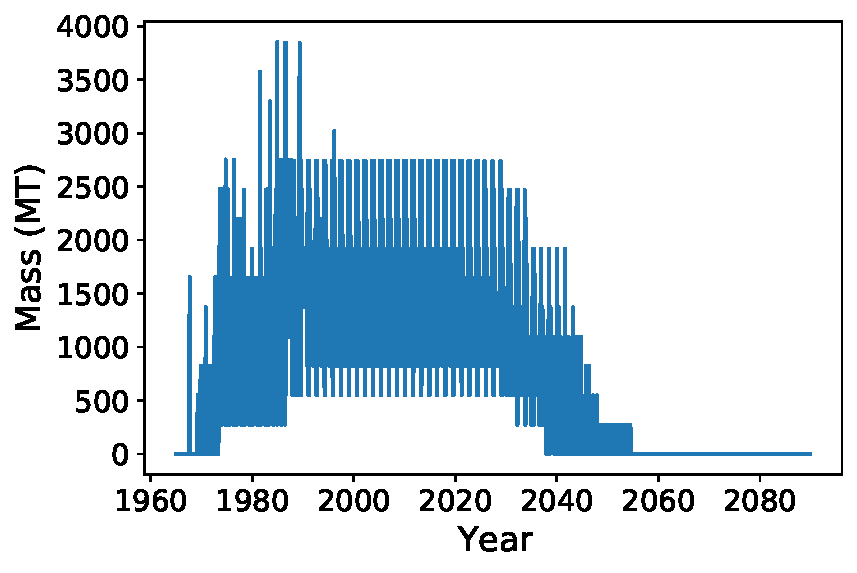
\includegraphics[scale=0.8]{s1_feed.pdf}
    \caption{Mass of natural uranium required to produce fuel for the LWRs at each 
    time step in Scenario 1.}
    \label{fig:feed1}
\end{figure}

The next metric of interest for this work is the \gls{SWU} capacity required 
to produce the enriched uranium for the \glspl{LWR}, 
shown in Figure \ref{fig:swu1}. This scenario requires a maximum of 3,714 
MT-SWU to 
enrich the uranium sent to the reactors at one time step and an average of 
981.4 MT-SWU/month to enrich all of the uranium sent to 
the \glspl{LWR} when they are deployed. An average of 
1192.4 MT-SWU/month is required to produce the enriched uranium 
for \glspl{LWR} between their initial deployment and 2025, and 
586.4 MT-SWU/month is needed to produce the 
enriched uranium sent to \glspl{LWR} between 2025 and 2055. The values 
reported here are different than what Bachmann et al. \cite{bachmann_enrichment_2021}
reports for a few different reasons. The first reason is that these results  
consider only
the time steps in which the \glspl{LWR} are deployed while Bachmann et al. 
considers all time steps. The other reason
is the use of different enrichment levels for the \gls{LWR} fuel. 
Bachmann et al. assumes an enrichment of 4.5\% while this work assumes 4.3\%
$^{235}$U enrichment for \gls{LWR} fuel. 


\begin{figure}
    \centering
    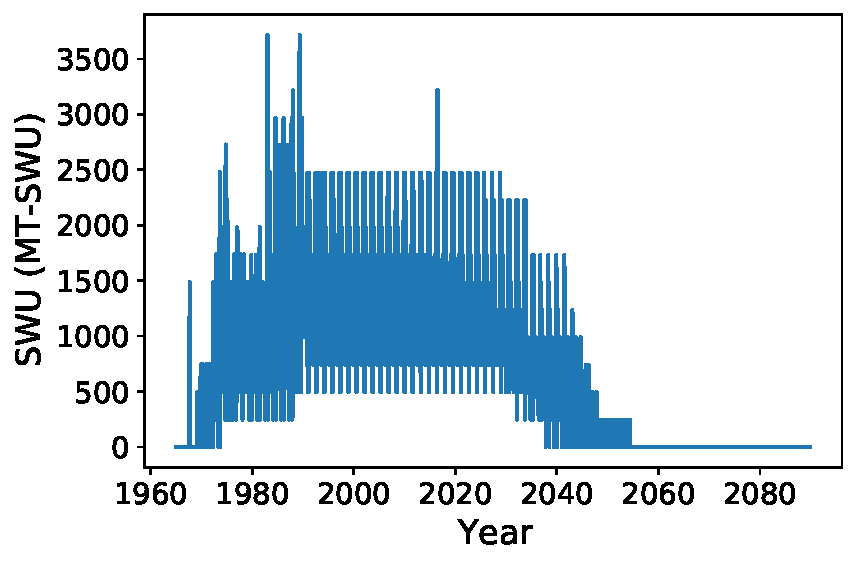
\includegraphics[scale=0.8]{s1_swu.pdf}
    \caption{SWU capacity required to enrich the uranium sent to LWRs at each time step in Scenario 1.}
    \label{fig:swu1}
\end{figure}

The last metric is the \gls{SNF} discharged from the reactors as a function of
time (Figure \ref{fig:waste1}). The \glspl{LWR} discharge a maximum of 393.6 MT 
of spent fuel in one time step and an average of 130.1 MT/month when they are 
deployed. Between the first \gls{LWR} deployment and 2025 the \glspl{LWR} 
discharge an average of 149.5 MTU/month, and an average of 93.9 MT/month  
between 2025-2055. The \glspl{LWR} discharge a total of 137,581 MT of \gls{SNF} 
in Scenario 1. 

\begin{figure}
    \centering
    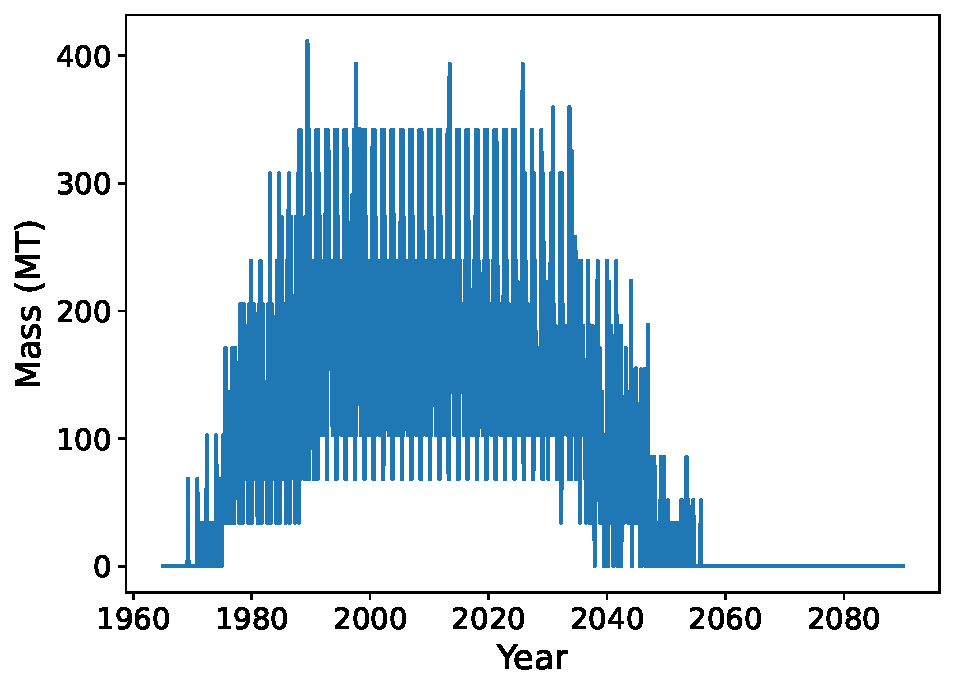
\includegraphics[scale=0.8]{s1_waste.pdf}
    \caption{Mass of spent fuel discharged from the reactors in Scenario 1 as a function of time.}
    \label{fig:waste1}
\end{figure}

\section{Energy Generated} \label{sec:energy}
This section reports and compares the energy produced in the no growth and 
1\% growth transition scenarios to the energy demand. This result 
considered the energy produced by \glspl{LWR} and advanced reactors. 

\subsection{No growth scenarios}
The energy demand in the no growth scenarios (Scenarios 2-7) is a constant
\hl{87.196} GWe-yr, based on the energy supplied by the reactors in Scenario 1
in 2025. The energy supplied in Scenarios 2-7 does not fully meet the demand
throughout the duration of the transition (Figure \ref{fig:nogrowth_energy}). 
This is because of a flaw in the modeling methodology. The advanced reactors 
are deployed to meet an installed capacity based on the energy generated by 
the \glspl{LWR}, which are not the same because of the capacity factor of 
each reactor. The initial gap between the energy produced and the demand results 
from the refueling of the \glspl{LWR}, but advanced reactors are not deployed 
yet because the installed capacity of the \glspl{LWR} is still greater than 
the energy produced. 

All of the 
transition scenarios experience the same energy production until 2030,
reaching a low point of 83.94 GWe-yr. Each of the scenarios exhibit 
variation 
in the annual energy production, which is a result of refueling 
periods for the \glspl{LWR} and any VOYGRs present. The maximum gap between 
energy production and demand is 5.406 GWe-yr, in Scenario 5 
(Table \ref{tab:nogrowth_energy}). There 
is very little oversupply of energy in any of these scenarios, with a 
maximum oversupply of 0.063 GWe-yr in Scenario 3. The overproduction of 
energy in Scenario 3 is a result of the advanced reactor deployment scheme 
of the transitions. For this scenario, Xe-100s are deployed until the 
installed capacity at least meets the demand. Therefore when dividing the 
energy demand by the capacity of the Xe-100 to determine the number of 
reactors to be deployed, the number is rounded up and the installed capacity 
is greater than the demand. Additionally, the Xe-100
has a capacity factor of 100\% in the simulations, therefore the energy
generated by the reactors matches their installed capacity. 

Throughout 
most of 2025-2090, Scenario 5 has the 
lowest energy 
production, producing between 84.05-85.20 GWe-yr. The lower energy 
production of Scenario 5 is because this scenario primarily deploys 
VOYGRs to meet the demand (Section \ref{sec:nogrowth_reactors}), which do 
not have a capacity factor of 100\%. Therefore the energy generated does 
not match the installed capacity and the energy generated does not meet the 
demand. 
Scenario 3 
produces the most energy, producing a constant 89.52 GWe-yr starting in 2056,
because the scenario only deploys the Xe-100, which has the largest 
power output  
and a capacity factor of 100\%.  Scenario 4 meets the 
energy demand the next best, producing a constant 89.46 GWe-yr starting in 
2056, because this scenario deploys Xe-100s and \glspl{MMR}. The 
Xe-100s meet most of the demand, because of their large power output.
The smaller power output of the \gls{MMR} allows for finer tuning of the 
installed capacity to the energy demand, compared with only deploying 
the Xe-100. Additionally, both of these reactors have a 100\% capacity 
factor, which means that the energy generated matches the installed capacity. 
The difference in power output in Scenarios 3 and 4 demonstrate how the 
\gls{MMR} can be used to better 
meet a specific power demand. 

\begin{figure}
    \centering
    \begin{subfigure}[b]{0.45\textwidth}
        \centering
        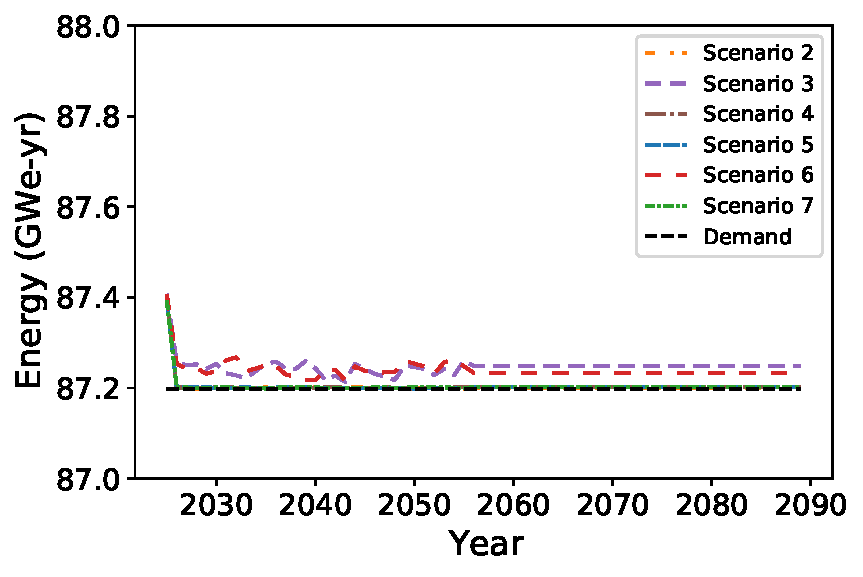
\includegraphics[width=\textwidth]{nogrowth_energy_after_2025.pdf}
        \caption{Annual energy produced compared to demand for Scenarios 2-7
        between 2025-2090.}
        \label{fig:nogrowth_energy_after_2025}
    \end{subfigure}
    \hfill
    \begin{subfigure}[b]{0.45\textwidth}
        \centering
        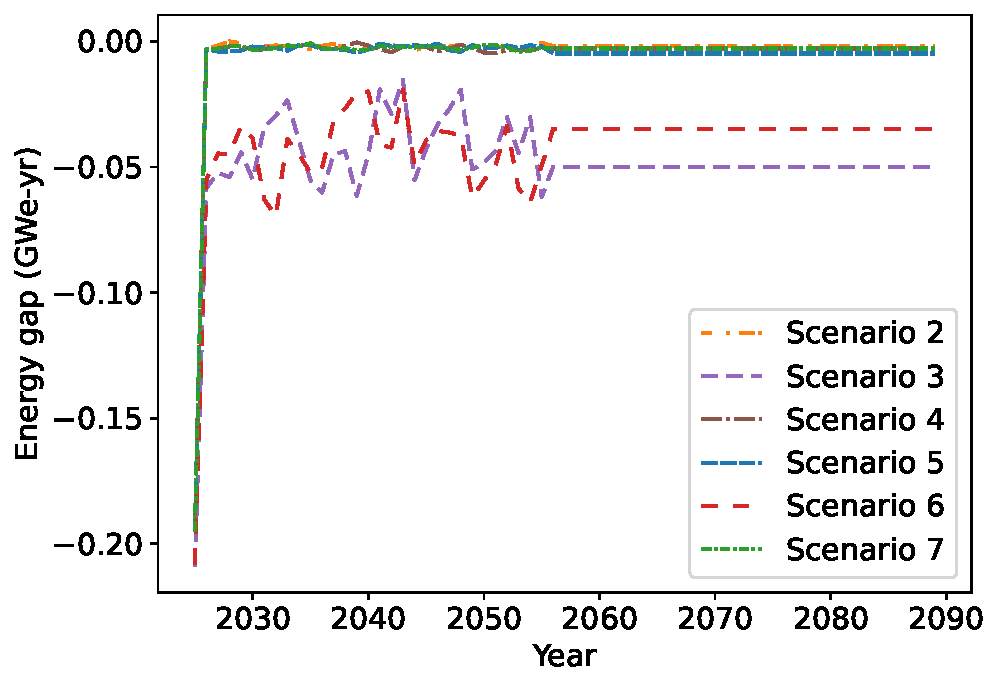
\includegraphics[width=\textwidth]{nogrowth_energy_gap.pdf}
        \caption{Gap between energy demand and energy produced by reactors 
        in Scenarios 2-7 between 2025-2090. Positive values indicate an 
        undersupply of energy and negative values represent an 
        oversupply of energy.}
        \label{fig:nogrowth_energy_gap}
    \end{subfigure}
       \caption{Annual energy produced compared to demand in Scenarios 2-7.}
       \label{fig:nogrowth_energy}
\end{figure}

\begin{table}
    \centering
    \caption{Maximum undersupply and oversupply of energy in Scenarios 2-7.}
    \label{tab:nogrowth_energy}
    \begin{tabular}{c c c}
        \hline 
        Scenario & Max Oversupply (GWe-yr) & Max Undersupply (GWe-yr) \\
        \hline 
        2 & 0.003 & 5.116 \\
        3 & 0.063 & 5.086 \\
        4 & 0.003 & 5.116 \\
        5 & 0.000 & 5.406 \\
        6 & 0.000 & 5.142 \\
        7 & 0.000 & 5.114 \\
        \hline
        
    \end{tabular}
\end{table}

\subsection{1\% growth scenarios}
For the 1\% growth scenarios there is a similar gap between energy 
production and 
demand immediately after the transition start time (Figure 
\ref{fig:1percent_energy}) to what was observed in the no growth 
scenarios. This gap is also because of this work's flawed methodology of 
matching an installed capacity to energy generated. All of the scenarios 
have an energy deficit 
between 2025 and the early 2050s, although Scenarios 11 and 12 never fully 
meet the energy demand. This deficit is because of the refueling 
requirements for the \glspl{LWR}, as the installed capacity from the 
\glspl{LWR} does not fall below the demand until 2027. Scenario 11
increases in the energy deficit with time, reaching a maximum deficit 
of 8.21 GWe-yr (Table \ref{tab:1percent_energy}). The energy deficit in 
Scenario 12 decreases with the other scenarios, then begins to increase 
in 2055, then begins to decrease again in 2087. The changes in the 
energy deficit are because of the rate of VOYGR deployment compared with 
the Xe-100 deployment (Section \ref{sec:1percent_reactors}). Around 2050
the rate of VOYGR deployment increases more than the rate of Xe-100 
deployment, causing VOYGRs to constitute a larger portion of the installed 
capacity. The VOYGR does not have a capacity factor of 100\% like the Xe-100 
though, so as more VOYGRs are built the gap between energy produced and 
energy demand increases. Around 2085 the number of VOYGRs built drops to 
0 and more Xe-100s are built. This change in which reactor is built decreases
the gap between energy produced and demand because the Xe-100 is modeled with 
a 100\% capacity factor, so as more are built the difference between installed 
capacity and energy generation decreases. 

The maximum gap between 
the energy demand and supply in any scenarios is 8.21 GWe-yr in Scenario 11, 
and the largest oversupply of energy in any of the scenarios is 
0.35 GWe-yr in Scenario 9 (Table \ref{tab:1percent_energy}). The large gap 
between demand and production in Scenario 11 is because this scenario mostly 
deploys VOYGRs (see Section \ref{sec:1percent_reactors} for further 
discussion), which do not 
have a capacity factor of 100\%. Scenario 9 produces a slight oversupply 
of energy because this scenario only deploys Xe-100s, which have the largest 
power output leading to the installed capacity being greater than the the 
energy demand. Since the Xe-100 has a capacity factor of 100\%, the energy 
produced is also greater than the energy demand. 

\begin{figure}
    \centering
    \begin{subfigure}[b]{0.45\textwidth}
        \centering
        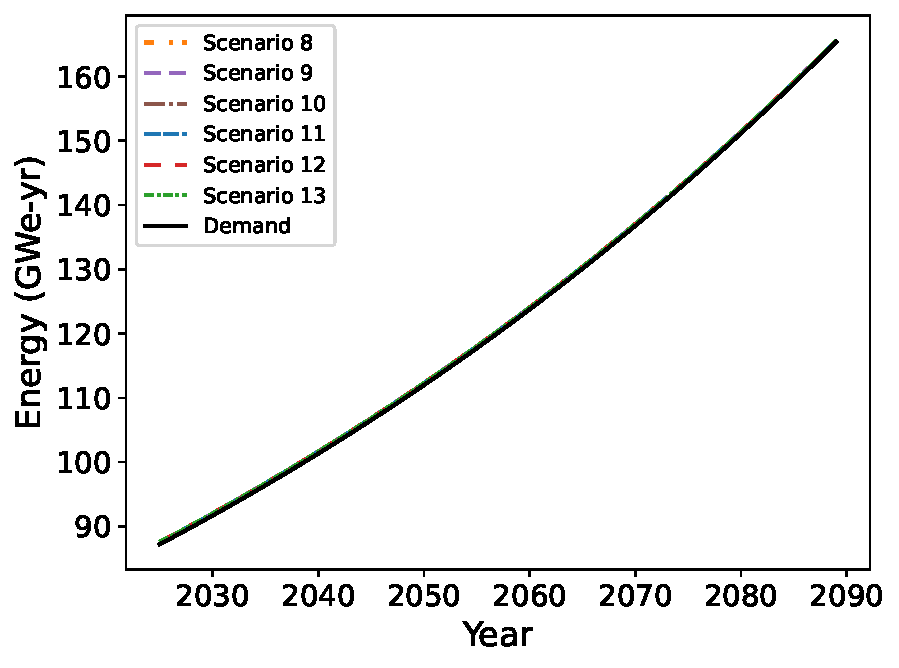
\includegraphics[width=\textwidth]{1percent_energy_after_2025.pdf}
        \caption{Annual energy produced compared to demand for Scenarios 8-13
        between 2025-2090.}
        \label{fig:1percent_energy_after_2025}
    \end{subfigure}
    \hfill
    \begin{subfigure}[b]{0.45\textwidth}
        \centering
        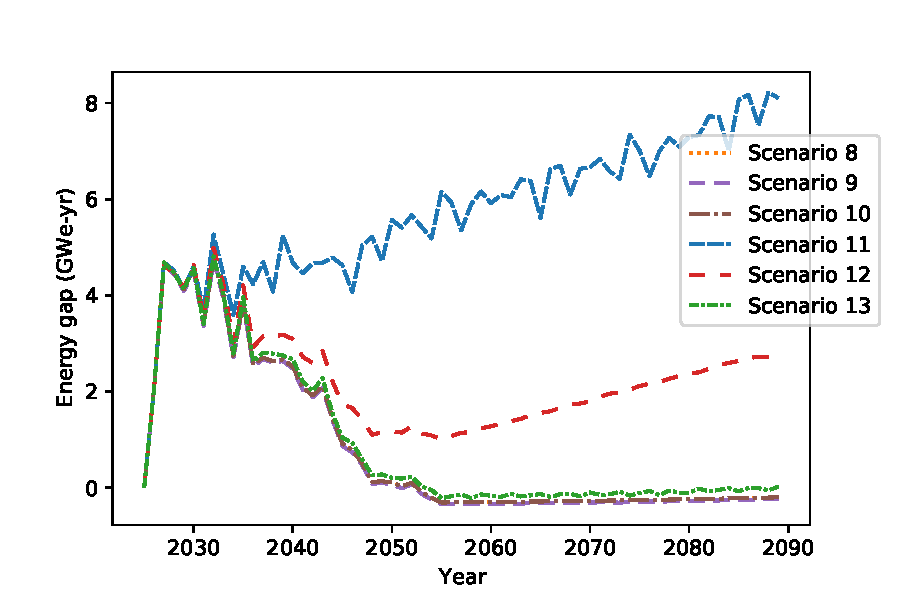
\includegraphics[width=\textwidth]{1percent_energy_gap.pdf}
        \caption{Gap between energy demand and energy produced in Scenarios 8-13
        between 2025-2090. Positive values represents an undersupply of energy 
        and negative values represents an oversupply of energy. }
        \label{fig:1percent_energy_gap}
    \end{subfigure}
       \caption{Annual energy produced compared to demand in Scenarios 8-13.}
       \label{fig:1percent_energy}
\end{figure}

\begin{table}
    \centering
    \caption{Maximum undersupply and oversupply of energy in Scenarios 8-13.}
    \label{tab:1percent_energy}
    \begin{tabular}{c c c}
        \hline 
        Scenario & Max Oversupply (GWe-yr) & Max Undersupply (GWe-yr) \\
        \hline 
        8 & 0.310 & 4.473 \\
        9 & 0.350 & 4.733 \\
        10 & 0.301 & 4.783 \\
        11 & 0.000 & 8.218 \\
        12 & 0.000 & 4.991 \\
        13 & 0.220 & 4.809\\
        \hline
        
    \end{tabular}
\end{table}

\section{Reactor deployment}
The different power output of each advanced reactor leads to different 
requirements in the number of advanced reactors deployed in each transition 
scenario. 
This section compares the scenarios on the number of advanced reactors 
built. This metric takes two 
different forms: the number of reactors that are in the simulation at 
one time and the number of reactors that are built (enter the simulation)
in a single time step. These metrics combined provide insight into the 
number of reactors needed and the rate at which to build them. 

\subsection{No growth scenarios} \label{sec:nogrowth_reactors}
Advanced reactors are first deployed in December 2029 for Scenario 2-7, 
about 5 years after transition start time. The delay between the start of 
the transition and the deployment of advanced reactors is because the 
advanced reactor deployment scheme is based on the installed capacity 
of the reactors and the
installed power capacity of the \glspl{LWR} is greater than the power demand
until December 2029. 
The advanced reactor initial deployment time is 
22 months earlier than the initial deployment time reported for no growth 
scenarios in 
\cite{bachmann_enrichment_2021} and one month earlier than the 
initial deployment time reported in \cite{bachmann_enrichment_2021}
for 1\% growth transitions. The differences in deployment times results 
from different deployment methods (Bachmann et al. used the \Cycamore 
\texttt{ManagerInst} institution to deploy advanced reactors), differences 
in information about the reactor designs, and a different energy demand 
(resulting from different assumptions of how long \glspl{LWR} operate). 

The number of reactors deployed varies based on 
the type of reactor used in the scenario and scales with the power output of 
each type of reactor, as shown in Figure \ref{fig:nogrowth_reactors}. Scenario
2 requires the most reactors, requiring 17,892 reactors at one time, 
because the \gls{MMR} has the smallest power output of the reactors 
considered in this work. Scenario 3 requires the fewest 
advanced reactors (1119) because this scenario only deploys the Xe-100,
which has the largest power output. The number of advanced reactors for 
these scenarios will not change if the deployment scheme is changed to 
match the advanced reactor energy generation to the energy demand because 
both of these reactors have capacity factors of 100\%. 

\begin{figure}
    \centering
    \begin{subfigure}[b]{0.45\textwidth}
        \centering
        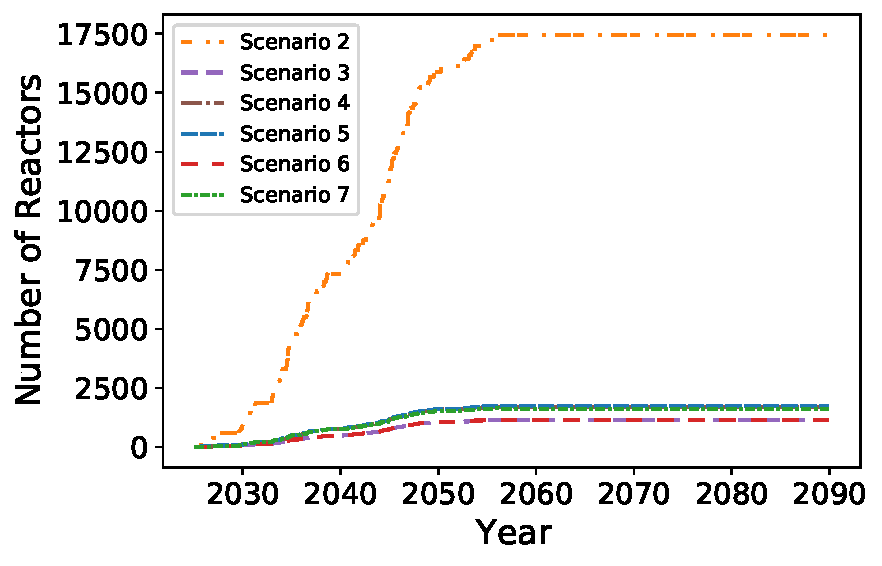
\includegraphics[width=\textwidth]{nogrowth_reactors.pdf}
        \caption{Total number of advanced reactors deployed at 
        each time step in Scenarios 2-7 between 2025-2090.}
        \label{fig:nogrowth_reactors_all}
    \end{subfigure}
    \hfill
    \begin{subfigure}[b]{0.45\textwidth}
        \centering
        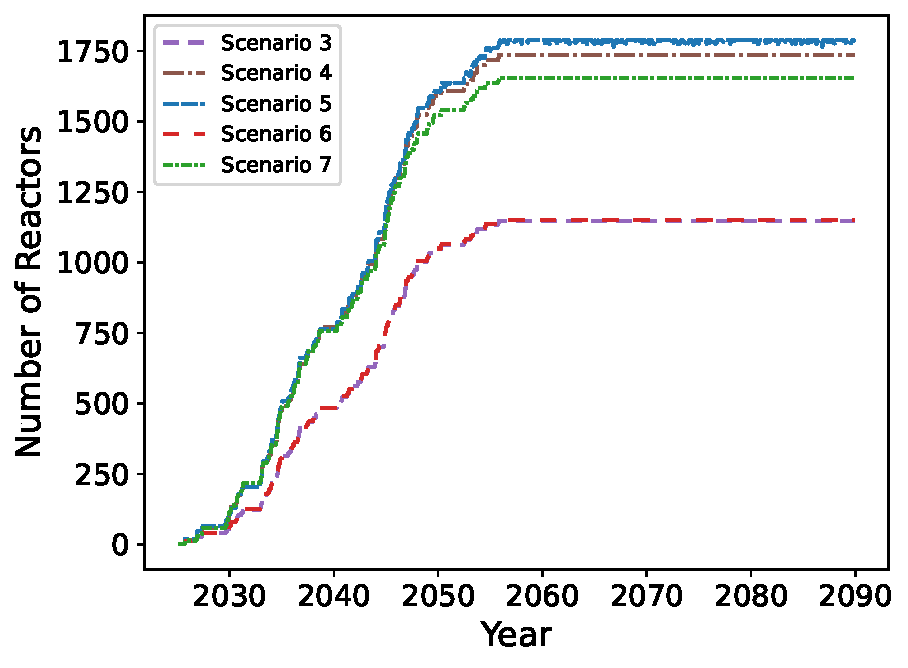
\includegraphics[width=\textwidth]{nogrowth_reactors_3-7.pdf}
        \caption{Total number of advanced reactors deployed at 
        each time step in Scenario 3-7 between 2025-2090.}
        \label{fig:nogrowth_reactors_3-7}
    \end{subfigure}
       \caption{Number of advanced reactors deployed at each time step 
       for Scenarios 2-7. The figures begin at 2025, because no advanced 
       reactors are deployed before then. In the right figure Scenario 
       2 is removed to highlight the trends in the other scenarios.}
       \label{fig:nogrowth_reactors}
\end{figure}

\begin{table}
    \centering 
    \caption{Maximum number of reactors deployed at one time in 
    Scenarios 2-7.}
    \label{tab:reactors_nogrowth}
    \begin{tabular}{c c c c c}
        \hline
        Scenario & \glspl{MMR} [\#] & Xe-100s [\#] & VOYGRs [\#] 
        & Total [\#]\\\hline
        2 & 17,892 & - & - & 17,892\\
        3 & - & 1,119 & - & 1,119\\
        4 & 628 & 1,079 & - & 1,707\\
        5 & 628 & - & 1,122 & 1,749\\
        6 & - & 1,045 & 77 & 1,122\\
        7 & 472 & 1,082 & 7 & 1,561\\
        \hline
    \end{tabular}
\end{table}

All of the scenarios have a constant number of advanced reactors 
deployed starting in October 2055 because all of the \glspl{LWR} are 
decommissioned by this time. The number of Xe-100s and VOYGRs combined 
in each scenario is similar, about 1,100, because these two reactor 
designs have similar power outputs (80 MWe and 77 MWe, respectively). 
Therefore, the deployment of one of these reactors over the others does 
not greatly affect the total number of them needed. However, 
deploying them in tandem reduces the number of \glspl{MMR} deployed
(Scenarios 4 and 5 compared with Scenario 7). If the deployment scheme 
is changed to match the advanced reactor energy generation to the demand, 
then the number of VOYGRs in each scenario is expected to increase because 
the VOYGR does not have a capacity factor of 100\% and therefore will 
generate less than 77 MWe-yr. 

In addition to the total number of each type of advanced reactor deployed 
at each time, the maximum number of each advanced reactor deployed in a 
single time step is reported in Table 
\ref{tab:reactors_added_nogrowth}. This information provides insight 
into the speed at which new reactors must be built. For scenarios with 
multiple advanced reactors, the numbers reported do not necessarily occur 
at the same time. Scenario 2 requires 
the largest number of reactors to be deployed at a single time, because 
the \gls{MMR} has the smallest power output. Scenarios 3 and 
6 deploy the fewest reactors in 
a single time step, based on the total column of Table 
\ref{tab:reactors_added_nogrowth}, because of the large power output from 
the Xe-100 and VOYGR. 

\begin{table}
    \centering 
    \caption{Maximum number of reactors added to the simulation at a 
    single time step in Scenarios 2-7.}
    \label{tab:reactors_added_nogrowth}
    \begin{tabular}{c c c c c}
        \hline
        Scenario & \glspl{MMR} [\#]& Xe-100s [\#]& VOYGRs [\#]
        & Total[\#]\\\hline
        2 & 756 & - & - & 756\\
        3 & - & 47 & - & 47\\
        4 & 16 & 47 & - & 54\\
        5 & 16 & - & 49 & 57\\
        6 & - & 46 & 2 & 47\\
        7 & 16 & 47 & 1 & 55\\
        \hline
    \end{tabular}
\end{table}

\subsection{1\% growth scenarios} \label{sec:1percent_reactors}
All of the 1\% growth scenarios deploy advanced reactors beginning 
in May 2027, which is 32 months (almost three years) before their initial 
deployment for a 1\% growth 
transition reported in \cite{bachmann_enrichment_2021} and 31 months 
earlier than for the no growth scenarios. If the deployment scheme is 
altered to be based on energy generated instead of installed capacity, 
then one would expect the initial deployment time to change. The number 
of reactors deployed in these scenarios is similar to 
the trends observed for the no 
growth scenarios. 

Transitioning to only the 
\gls{MMR} (Scenario 8) requires the largest number of reactors, and 
transitioning to only the Xe-100 (Scenario 9) requires the fewest 
number of advanced reactors (Figure \ref{fig:1percent_reactors}, Table 
\ref{tab:reactors_1percent}). Scenarios 10 and 13 have similar numbers of 
reactors deployed, as do Scenarios 9 and 12, because these pairing differ 
by the inclusion of the VOYGR which has a similar power output to the 
Xe-100. However, because of the lower capacity factor of VOYGRs more will 
need to be built to actually meet the energy demand. 
Compared with the no growth scenarios, \glspl{MMR} are a greater 
fraction of the total number of reactors deployed when they are deployed 
with the other reactors (Scenarios 10, 11, and 13). This increase is 
because early in the transition the growth of the energy demand 
changes in increments smaller than the power output of the Xe-100 and 
VOYGR. Therefore, the deployment scheme of this work dictates the 
deployment of \glspl{MMR}
to fulfill the unmet demand. Scenarios 10, 11, and 13 exhibit decreases in 
the number of advanced reactors deployed between 2045-2055 as the unmet 
demand, resulting from the growth in the demand, the decommissioning of 
\glspl{LWR}, and the decommissioning of \glspl{MMR}, increases  
to an amount that can be met by deploying new Xe-100s and VOYGRs. Therefore, 
the total number of advanced reactors deployed in the simulation decreases.

\begin{figure}
    \centering
    \begin{subfigure}[b]{0.45\textwidth}
        \centering
        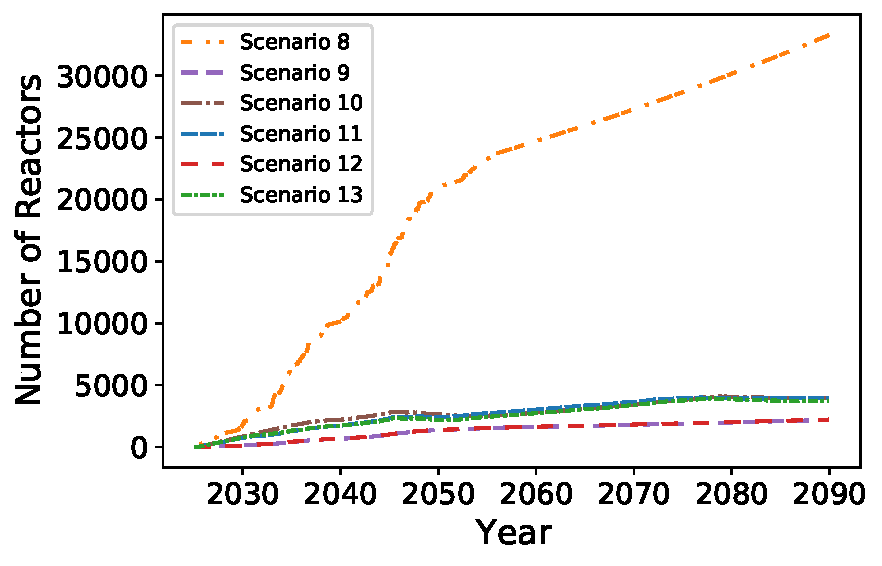
\includegraphics[width=\textwidth]{1percent_reactors.pdf}
        \caption{Total number of advanced reactors deployed at 
        each time step in Scenarios 8-13 between 2025-2090.}
        \label{fig:1percent_reactors_all}
    \end{subfigure}
    \hfill
    \begin{subfigure}[b]{0.45\textwidth}
        \centering
        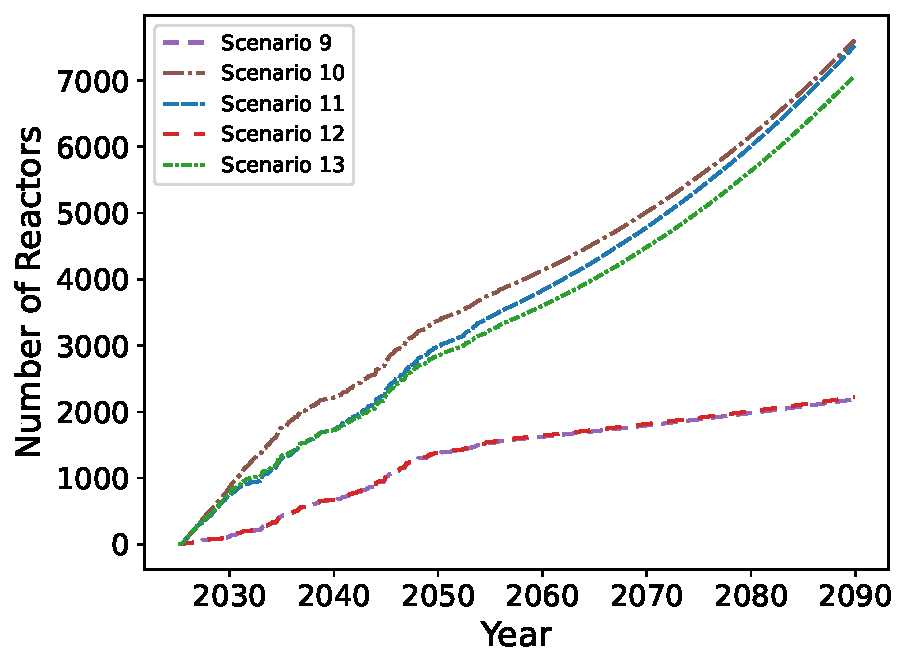
\includegraphics[width=\textwidth]{1percent_reactors_9-13.pdf}
        \caption{Total number of advanced reactors deployed at 
        each time step in Scenario 9-13 between 2025-2090.}
        \label{fig:1percent_reactors_9-13}
    \end{subfigure}
       \caption{Number of advanced reactors deployed at each time step 
       for Scenarios 8-13. The figures begin at 2025, because no advanced 
       reactors are deployed before then. In the right figure Scenario 
       8 is removed to help highlight the trends in the other scenarios.}
       \label{fig:1percent_reactors}
\end{figure}

\begin{table}
    \centering 
    \caption{Maximum number of advanced reactors deployed in Scenarios 8-13.}
    \label{tab:reactors_1percent}
    \begin{tabular}{c c c c c}
        \hline
        Scenario & \glspl{MMR} [\#]& Xe-100s [\#]& VOYGRs [\#] 
        & Total [\#]\\\hline
        8 & 34,126 & - & - & 34,126\\
        9 & - & 2,139 & - & 2,139 \\
        10 & 2,494 & 2,004 & - & 4,299\\
        11 & 2,333 & - & 2,096 & 4,143\\
        12 & - & 1,418 & 749 & 2,167\\
        13 & 2,320 & 1,976 & 46 & 4,114\\
        \hline
    \end{tabular}
\end{table}

Regarding the rate of reactor deployment, Scenario 8 deploys the most 
reactors in a single time step (Table 
\ref{tab:reactors_added_1percent}), with 832 \glspl{MMR} deployed at once. 
Scenario 11 requires the next largest number of reactors deployed in 
a single time step, 50 VOYGRs in one step and 60 total advanced reactors. 
Scenarios 9 and 12 require the same total number of advanced reactors 
deployed in the same time step. With the exception of Scenario 8, each of 
the 1\% growth scenarios require a similar maximum number of advanced 
reactors deployed in a single time step as the corresponding no growth 
scenario (e.g., Scenarios 3 and 9). 

\begin{table}
    \centering 
    \caption{Maximum number of advanced reactors deployed in a single 
    time step for Scenarios 8-13.}
    \label{tab:reactors_added_1percent}
    \begin{tabular}{c c c c c}
        \hline
        Scenario & \glspl{MMR} [\#] & Xe-100s [\#] & VOYGRs [\#] 
        & Total [\#]\\\hline
        8 & 823 & - & - & 823\\
        9 & - & 49 & - & 49\\
        10 & 16 & 48 & - & 57\\
        11 & 16 & - & 50 & 60\\
        12 & - & 48 & 2 & 49\\
        13 & 16 & 48 & 1 & 57\\
        \hline
    \end{tabular}
\end{table}

\section{Uranium resources}
This metric considers  
both the mass of enriched uranium and the mass of natural uranium feed 
required by each scenario. The feed uranium masses 
considered are the masses needed at an enrichment facility,
and does not account for any process losses between mining and 
enrichment. Therefore, the values reported are not the same as what would 
need to be mined. Additionally, the masses reported do not account for 
any fuel fabrication losses, which others have previously assumed to 
be 0.1\% \cite{wigeland_nuclear_2014}. 

The masses of uranium resources are divided into four 
different metrics: the average monthly mass of uranium to supply all 
advanced reactors, the average monthly mass of \gls{HALEU}, the 
maximum mass of uranium required by all advanced 
reactors in a single time step, and the cumulative mass required by the 
scenario. Each of these metrics provide information 
on how to design facilities, such as the average facility capacity 
required to meet the average demand and peaks in demand. The monthly 
averages are calculated beginning in January 2025, 
when the transition begins but not when the advanced reactors 
are first deployed. Therefore, the reported averages are slightly lower 
than if they were calculated starting at the advanced reactor deployment 
time. This reporting methodology provides an average for if 
facilities are built to support the front-end of the \gls{NFC} starting 
in January 2025. 

\subsection{No growth scenarios}
The mass of enriched uranium sent to reactors (Fig. \ref{fig:nogrowth_uranium})
varies based on the advanced reactors deployed in the scenario. 
Scenario 5 has the largest average mass of enriched uranium sent to 
reactors each month, followed by Scenario 2 (Table 
\ref{tab:nogrowth_uranium}). 
Scenario 2 also requires the largest mass of enriched uranium sent 
to advanced reactors at one time, followed by Scenario 5.
Scenario 3 requires the smallest average 
mass of enriched uranium. Scenarios 3, 4, and 7 
have similar monthly averages for enriched uranium mass. All of the 
scenarios require a smaller 
average mass of enriched uranium than the \glspl{LWR} before 2025. 

The uranium usage of each advanced reactor dictates the uranium requirements 
of each scenario. The \gls{MMR} has the smallest specific power (thermal 
power per unit mass) for a single core mass and the Xe-100 has the largest 
specific power. This metric means that to meet the same thermal power 
output, the Xe-100 will require the least uranium mass, followed by the 
VOYGR then the \gls{MMR}. However, this does not include any fuel needed for 
refueling. The \gls{MMR} does not need any uranium for refueling, but the 
Xe-100 and VOYGR do. The Xe-100 requires a smaller mass for each refueling 
than the VOYGR and a smaller mass over the same amount of time. Therefore, 
the VOYGR requires the most mass over a given period of time to produce 
a certain amount of power (accounting for refueling schemes and power  
output). This larger mass requirement of the VOYGR leads to the 
masses required by Scenario 5, 
which primarily deploys VOYGRs.

Comparing the \gls{MMR} and Xe-100 requires less uranium than the \gls{MMR}, 
and the least of all three advanced reactors, over a given period of time 
to produce a given amount of power. This reduced uranium mass results 
from the high burnup of the Xe-100, so the reactor gets more energy out of 
each mass of fuel and has a larger power output. This reduced uranium mass 
required by the Xe-100 leads to Scenario 3, which only deploys the 
Xe-100, to require the least uranium. Scenarios 4, 6, and 7 require similar 
masses of uranium because Xe-100s constitute a majority of the advanced 
reactors deployed and largely control the uranium required. 

\begin{figure}
    \centering
    \begin{subfigure}[b]{0.45\textwidth}
        \centering
        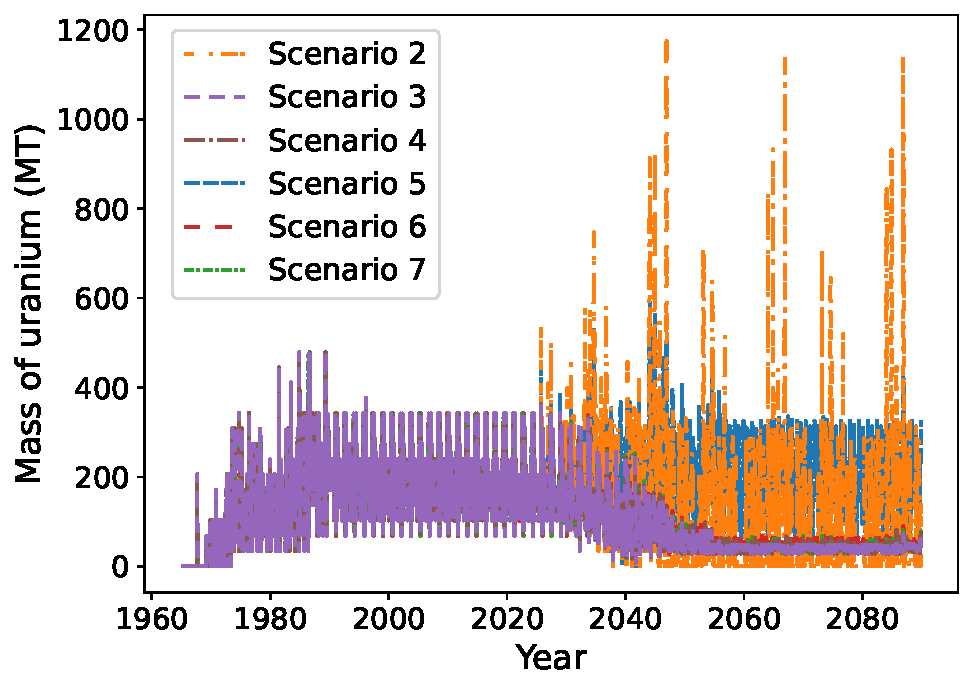
\includegraphics[width=\textwidth]{nogrowth_uranium.pdf}
        \caption{Monthly mass of enriched uranium sent to all reactors 
        between 1965-2090.}
        \label{fig:nogrowth_all_uranium}
    \end{subfigure}
    \hfill
    \begin{subfigure}[b]{0.45\textwidth}
        \centering
        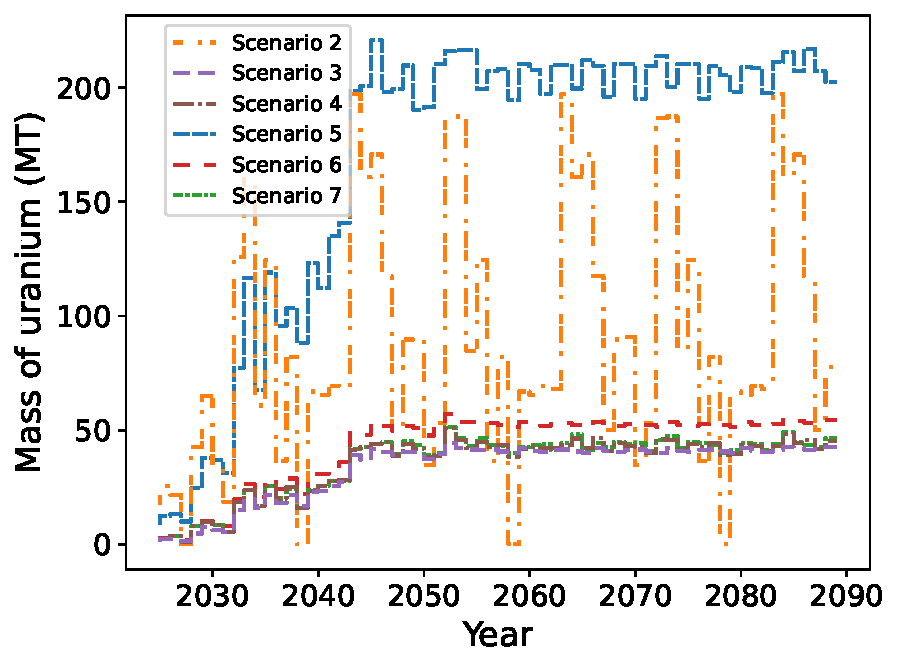
\includegraphics[width=\textwidth]{nogrowth_AR_uranium.pdf}
        \caption{Annual average mass of enriched uranium sent to 
        advanced reactors between 2025-2090.}
        \label{fig:nogrowth_AR_uranium}
    \end{subfigure}
    \begin{subfigure}[b]{0.45\textwidth}
        \centering
        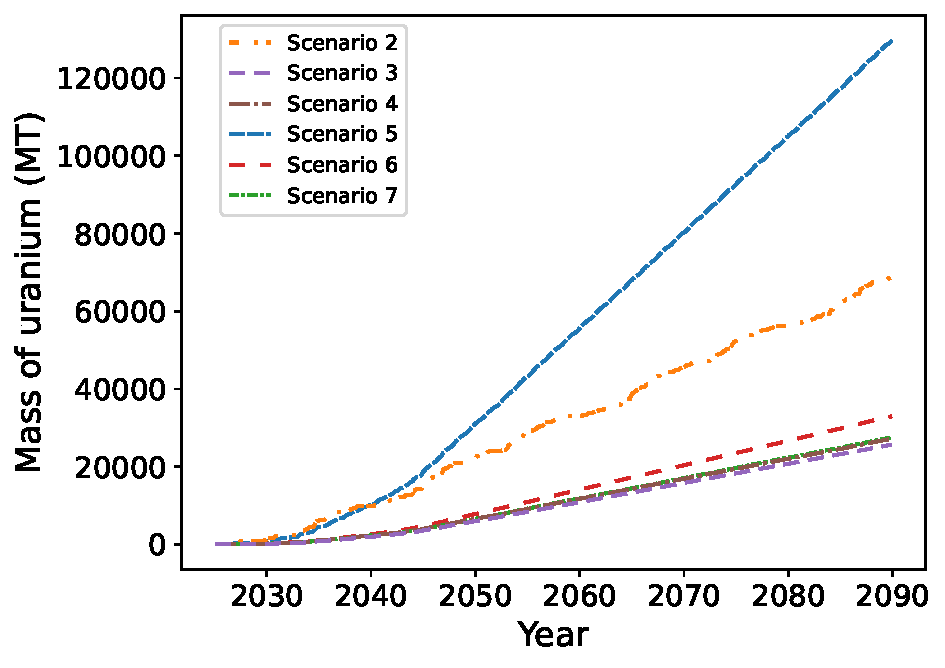
\includegraphics[width=\textwidth]{nogrowth_uranium_cumulative.pdf}
        \caption{Cumulative mass of enriched 
        uranium sent to advanced reactors between 2025-2090.}
        \label{fig:nogrowth_uranium_cumulative}
    \end{subfigure}
       \caption{Mass of enriched uranium required by reactors
        in Scenarios 2-7.}
       \label{fig:nogrowth_uranium}
\end{figure}

\begin{table}
    \centering 
    \caption{Metrics for enriched uranium sent to advanced 
    reactors between 2025-2090 in Scenarios 2-7.}
    \label{tab:nogrowth_uranium}
    \begin{tabular}{c c c c c}
        \hline
        Scenario & Average (MT/month) & \gls{HALEU} Average 
        (MT/month) & Maximum (MT)& Cumulative (MT)\\\hline
        2 & 88.90 & 88.90 & 1,007 & 69,251\\
        3 & 31.64 & 31.64 & 86.79 & 24,646\\
        4 & 33.62 & 33.62 & 101.5 & 26,193\\
        5 & 152.3 & 3.070 & 581.1 & 118,608\\
        6 & 39.92 & 29.51 & 103.3 & 31,095\\
        7 & 33.85 & 32.97 & 103.0 & 26,370\\
        \hline
    \end{tabular}
\end{table}

Scenario 2 requires the largest average mass of \gls{HALEU}, because 
of the large number of \glspl{MMR} deployed in this scenario. Scenario 
5 requires the smallest average mass of \gls{HALEU}, despite requiring the 
largest average mass of enriched uranium, because most of the 
reactors in Scenario 5 are VOYGRs which do not require \gls{HALEU}. 
All of the other scenarios (Scenarios 3, 4, 6, and 7) require similar 
average masses of uranium and \gls{HALEU} because they deploy similar 
numbers for each type of reactor. 

Scenarios 2 and 5 require the largest mass of enriched uranium at a single 
time step. For Scenario 2, the large difference between the average and 
maximum amount of uranium is because of the refueling scheme for the 
\gls{MMR}. The \gls{MMR} only requires fuel when it is first being 
commissioned, therefore they do not require uranium at time periods in 
which
new reactors are not deployed. The \gls{MMR} refueling scheme also 
causes the variation in the monthly requirements and annual averages of 
enriched uranium masses. The large difference between the 
monthly average and the maximum presents challenges in designing enrichment 
and fuel fabrication facilities 
to meet the demand. Designing such facilities would have to consider the 
material demands while also limiting the amount of stockpiled enriched 
uranium at each the facility, as idle stockpiles of enriched uranium 
poses a proliferation risk. 

Finally, Scenario 5 requires the largest cumulative mass of enriched uranium 
for the no growth scenarios, which is consistent with Scenario 5 requiring 
the largest average monthly mass of enriched uranium.  Scenario 3 requires 
the smallest cumulative 
mass of enriched uranium, which is consistent with this scenario requiring 
the smallest average mass. The advanced reactors 
in all of these scenarios require a smaller cumulative mass of fuel than 
the \glspl{LWR}. Additionally, deploying the VOYGR in tandem with the other 
advanced reactors results in an increase in the cumulative mass 
of enriched uranium needed (e.g., Scenario 3 compared with Scenario 6). This
trend suggests that deploying VOYGRs increases the enriched uranium needs 
of the fuel cycle, even if it decreases the amount of \gls{HALEU} needed. 

The cumulative \gls{HALEU} need by 2050 for each scenario (Table 
\ref{tab:nogrowth_haleu}) is similar to the mass reported by 
Dixon et al. \cite{dixon_estimated_2022}, 5350 MTU, with the exception 
of Scenarios 2 and 5. Scenario 2 requires a greater cumulative mass of 
\gls{HALEU} because of the large number of \glspl{MMR} deployed. Scenario 
5 requires a much lower mass of \gls{HALEU} because this scenario mostly 
deploys VOYGRs. 

\begin{table}
    \centering 
    \caption{Cumulative HALEU needs by 2050 for Scenarios 2-7.}
    \label{tab:nogrowth_haleu}
    \begin{tabular}{c c}
        \hline 
        Scenario & Cumulative mass (MT) \\
        \hline
        2 & 21,745\\
        3 & 5,500 \\
        4 & 6,080 \\
        5 & 764 \\
        6 & 5,111 \\
        7 & 5,913 \\
        \hline        
    \end{tabular}
\end{table}

For the mass of feed uranium, Scenario 2 requires the largest average mass 
to supply the advanced reactors (Figure \ref{fig:nogrowth_feed}, Table 
\ref{tab:nogrowth_feed}). Scenario 2 requires the most feed uranium 
because it requires a larger mass of enriched uranium than most 
of the other no growth scenarios and it requires the largest product 
assay. As Eq. \ref{eq:enrichment_assasys} shows, as the product assay 
increases, the mass of feed uranium increases, assuming all other 
variables are constant. Scenario 5 requires the next largest average 
mass of feed uranium, and requires less feed uranium than Scenario 2 
because 
most of the product uranium for this scenario is for the VOYGRs, which 
require a lower enrichment assay than the \glspl{MMR}. Based on Eq. 
\ref{eq:enrichment_assasys}, a lower assay of the product stream results in 
a lower mass of feed material required. Scenario 5 still requires more feed 
material than the other scenarios because the average product mass required 
is much larger than the other scenarios, which offsets some of the decrease 
in feed material from the decrease in the product assay. 

\begin{figure}
    \centering
    \begin{subfigure}[b]{0.45\textwidth}
        \centering
        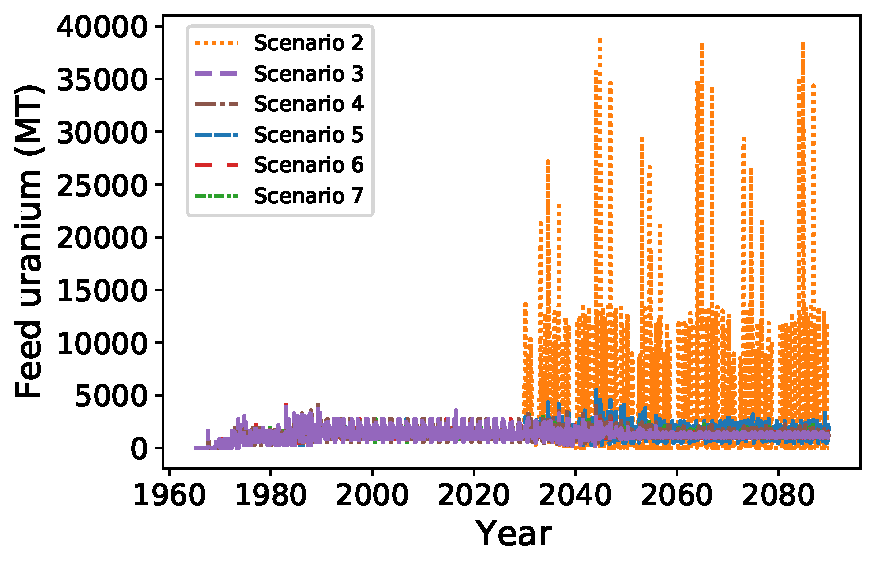
\includegraphics[width=\textwidth]{nogrowth_feed.pdf}
        \caption{Monthly mass of feed uranium to produce enriched uranium sent to 
        all reactors between 1965-2090.}
        \label{fig:nogrowth_all_feed}
    \end{subfigure}
    \hfill
    \begin{subfigure}[b]{0.45\textwidth}
        \centering
        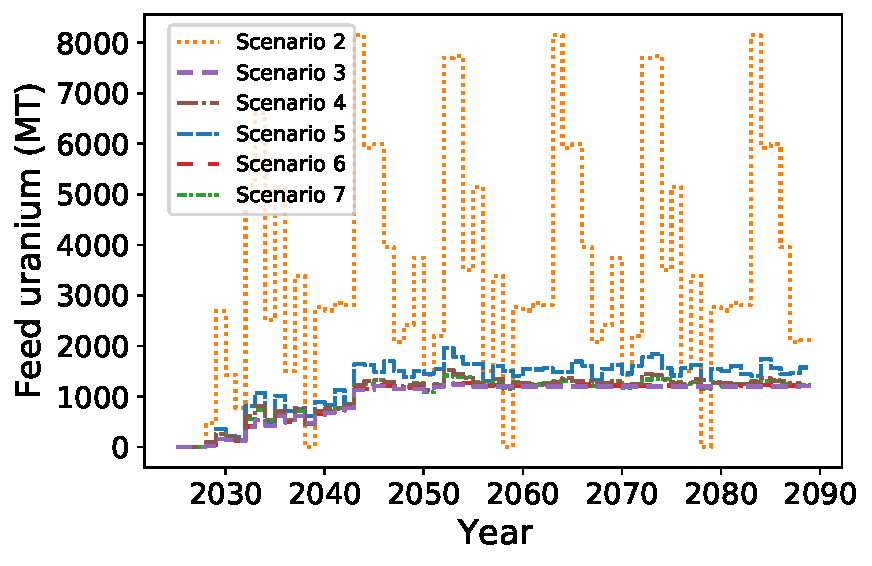
\includegraphics[width=\textwidth]{nogrowth_AR_feed.pdf}
        \caption{Annual average mass of feed uranium to produce enriched uranium sent to 
        advanced reactors between 2025-2090.}
        \label{fig:nogrowth_AR_feed}
    \end{subfigure}
    \begin{subfigure}[b]{0.45\textwidth}
        \centering
        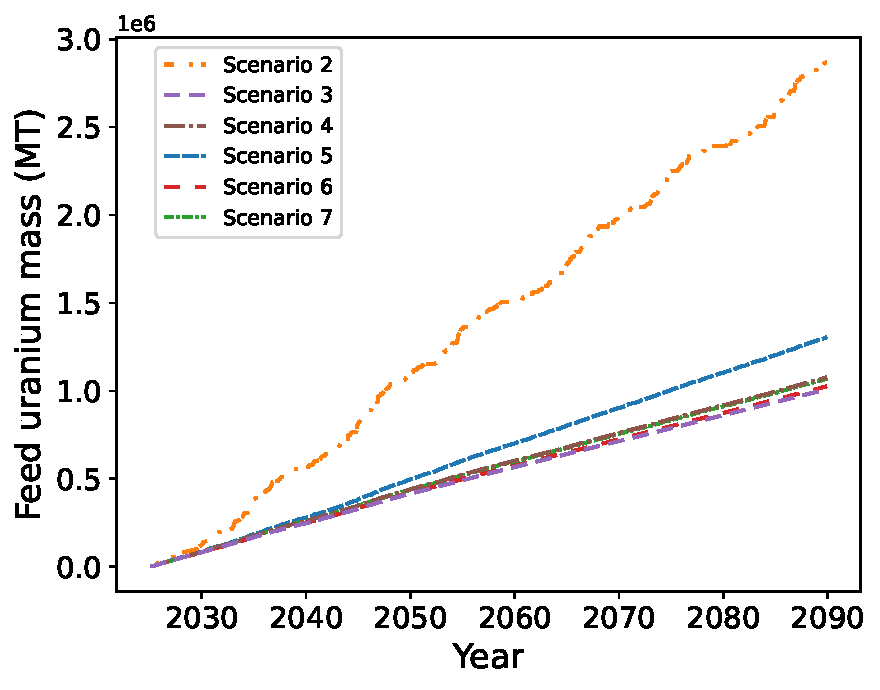
\includegraphics[width=\textwidth]{nogrowth_feed_cumulative.pdf}
        \caption{Cumulative mass of feed uranium to produce enriched 
        uranium for advanced reactors between 2025-2090.}
        \label{fig:nogrowth_feed_cumulative}
    \end{subfigure}
       \caption{Mass of feed uranium required to produce enriched uranium
        in Scenarios 2-7.}
       \label{fig:nogrowth_feed}
\end{figure}

\begin{table}
    \centering 
    \caption{Metrics for feed uranium required by advanced reactors 
    between 2025-2090 in Scenarios 2-7.}
    \label{tab:nogrowth_feed}
    \begin{tabular}{c c c c c}
        \hline
        Scenario & Average (MT/month) & \gls{HALEU} Average 
        (MT/month) & Maximum (MT) & Cumulative (MT)\\\hline
        2 & 3,401 & 3,401 & 38,517 & 2,649,436\\
        3 & 947.3 & 947.3 & 2,598 & 737,950\\
        4 & 1,032 & 1,032 & 3,171 & 804,647\\
        5 & 1,253 & 117.5 & 4,668 & 976,207\\
        6 & 962.9 & 883.7 & 2,681 & 750,072\\
        7 & 1,013 & 1,007 & 3,228 & 789,745\\
        \hline
    \end{tabular}
\end{table}

When comparing the feed material to create \gls{HALEU} in each scenario, 
Scenario 2 requires the most feed material because this scenario 
requires the largest average mass of \gls{HALEU} and \gls{HALEU} at the 
highest product assay. Scenario 5 requires the least feed material for 
\gls{HALEU} because the majority of 
the reactors in this scenario are VOYGRs.
Additionally, fueling the Xe-100 requires less feed uranium than fueling 
the \gls{MMR} because the Xe-100 requires a lower product assay and a 
smaller product mass per core. 
Scenarios 3, 4, and 7 require similar feed uranium masses (about 1,000 
MTU/month). Deploying VOYGRs alongside the other advanced 
reactors (e.g., between Scenarios 3 and 6) decreases the average 
mass of feed uranium to create \gls{HALEU}. Deploying VOYGRs decreases the 
average of all feed uranium if \glspl{MMR} are also deployed, because the 
decrease in product assay between these reactors offsets the increase in 
total product mass when calculating the feed mass. 

The maximum feed uranium required by each scenario poses some 
challenge in facility design. The maximum feed uranium required varies 
between 2.7-14.8 times larger than the average feed material, which means 
that 
facilities to produce feed uranium will likely need to be designed with a 
larger capacity than the average feed uranium required to meet the peaks. 
The cumulative mass of feed uranium required by each scenario ranges between 
737,000-978,000 MTU for every scenario except Scenario 2. 
Scenario 2 requires over 2.64 million MTU, which is more feed uranium 
than what is required by the \glspl{LWR}. The \gls{EIA} reports 
about 176,000 MT of U$_3$O$_8$ reserves in the US available at up to 
\$100/pound at the end of 2019 \cite{us_eia_2020_2021}, or about 
149,000 MT of uranium, which is smaller than the cumulative needs for 
all of these scenarios. Therefore, the US must consider either uranium 
from international sources or uranium reserves at increased 
prices to meet the cumulative demand of feed 
uranium for each of these scenarios.

\subsection{1\% growth scenarios}
The trends observed in the 1\% growth scenarios match the trends 
observed with the no growth scenarios that deploy the same reactor 
types
(Figure \ref{fig:1percent_uranium} and Table \ref{tab:1percent_uranium}). 
Scenario 11 requires the largest average mass of enriched uranium, and Scenario
8 requires the next largest average. Scenario 8 requires the largest 
average mass of \gls{HALEU}, while Scenario 11 requires the least, and the 
other scenarios require less than 56 MT/month. Scenario 9 requires the 
smallest monthly average of enriched uranium, because this scenario 
deploys the least number of reactors, and the Xe-100 requires the smallest 
mass of fuel in the core. 

\begin{figure}
    \centering
    \begin{subfigure}[b]{0.45\textwidth}
        \centering
        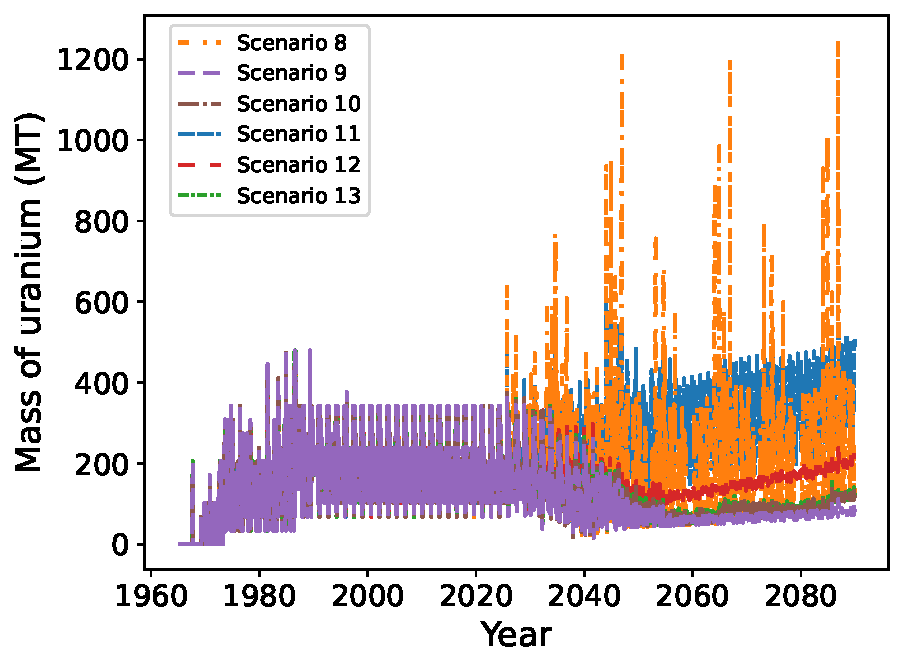
\includegraphics[width=\textwidth]{1percent_uranium.pdf}
        \caption{Mass of uranium sent to all reactors between 1965-2090.}
        \label{fig:1percent_all_uranium}
    \end{subfigure}
    \hfill
    \begin{subfigure}[b]{0.45\textwidth}
        \centering
        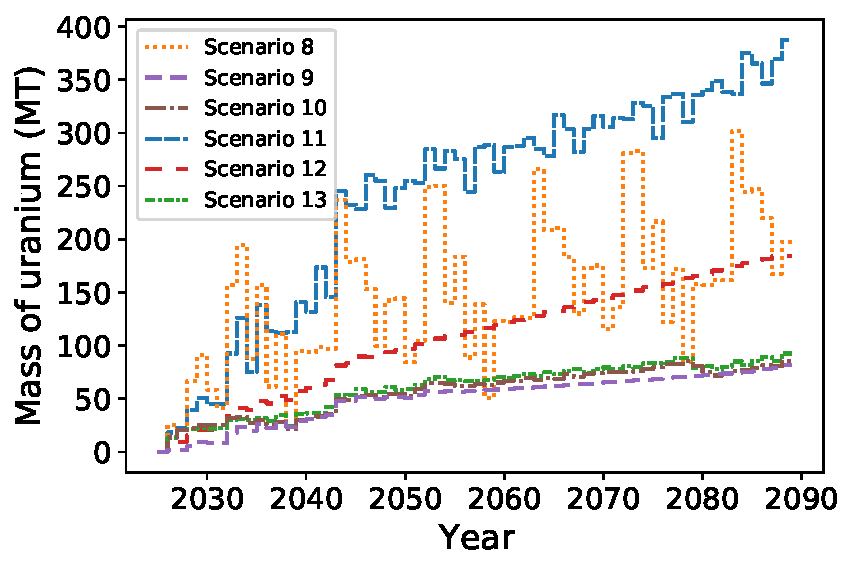
\includegraphics[width=\textwidth]{1percent_AR_uranium.pdf}
        \caption{Annual average mass of enriched uranium sent to 
        advanced reactors between 2025-2090.}
        \label{fig:1percent_AR_uranium}
    \end{subfigure}
    \begin{subfigure}[b]{0.45\textwidth}
        \centering
        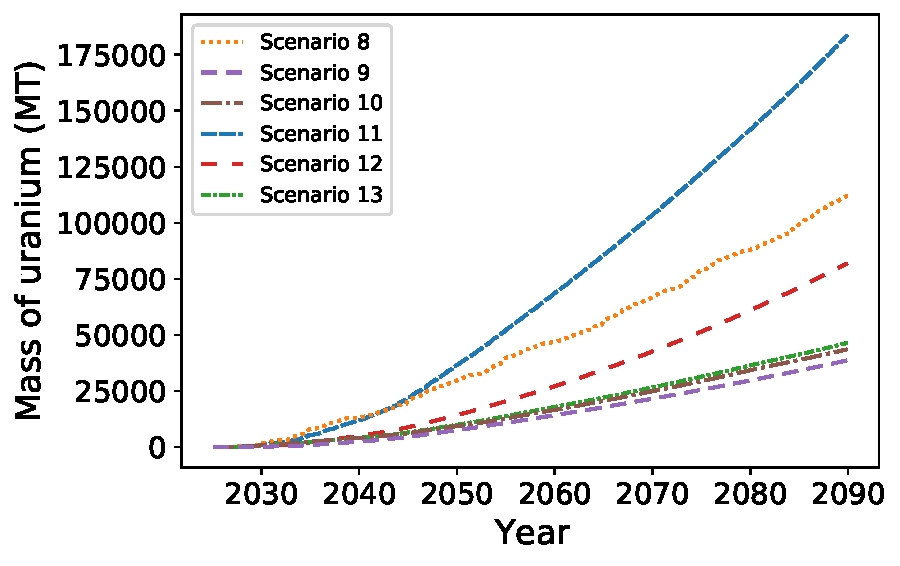
\includegraphics[width=\textwidth]{1percent_uranium_cumulative.pdf}
        \caption{Cumulative mass of enriched uranium sent to advanced reactors 
        between 2025-2090.}
        \label{fig:1percent_uranium_cumulative}
    \end{subfigure}
       \caption{Mass of enriched uranium required by reactors
        in Scenarios 8-13.}
       \label{fig:1percent_uranium}
\end{figure}

\begin{table}
    \centering 
    \caption{Metrics for enriched uranium required by advanced reactors 
    between 2025-2090 in Scenarios 8-13.}
    \label{tab:1percent_uranium}
    \begin{tabular}{c c c c c}
        \hline
        Scenario & Average (MT/month) & \gls{HALEU} Average  
        (MT/month) & Maximum (MT) & Cumulative (MT)\\\hline
        8 & 143.8 & 143.8 & 1,096 & 112,054\\
        9 & 49.65 & 49.65 & 98.36 & 38,679\\
        10 & 55.95 & 55.95 & 109.9 & 43,583\\
        11 & 235.9 & 9.314 & 616.2 & 183,730\\
        12 & 105.1 & 35.48 & 200.2 & 81,907\\
        13 & 59.60 & 54.17 & 115.5 & 46,431\\
        \hline
    \end{tabular}
\end{table}

The maximum mass of enriched uranium required in each scenario ranges 
between 2.0-7.6 times the average monthly mass, which is a smaller increase 
than for the no growth scenarios. The increase between 
the average and the maximum is smaller for the 1\% growth scenarios because
the averages increase more than the maximums for the scenarios deploying the 
same reactors (e.g., between Scenarios 2 and 8). The cumulative mass 
of enriched uranium required has a similar pattern to the average mass;
Scenario 11 requires the most mass, followed by Scenario 8. Scenario 
9 requires the least cumulative mass. 
The advanced reactors in Scenario 11 require more enriched uranium 
than the \glspl{LWR}, but the other scenarios require less than the 
\glspl{LWR}. 

The trends of the mass of feed uranium required by Scenarios 8-13 (Figure \ref{fig:1percent_feed},
Table \ref{tab:1percent_feed}) is consistent with trends of the feed 
requirements of the no growth scenarios. Scenario 8 requires the 
most feed uranium based on any of the metrics in Table 
\ref{tab:1percent_feed}, because of the larger number of 
reactors deployed than the other scenarios and all of the reactors deployed 
require \gls{HALEU}. The larger product assay of \gls{HALEU}, compared with 
the product assay for \glspl{LWR} or VOYGRs, means that more 
feed uranium is needed to produce the same product mass (Eq. 
\ref{eq:enrichment_assasys}). Scenario 11 requires the next largest amount 
of 
feed uranium, with most of the feed uranium used to produce enriched 
uranium for the VOYGRs. The other scenarios require similar monthly 
averages of feed uranium, with Scenario 9 requiring the least amount of 
feed uranium. To produce \gls{HALEU}, Scenario 8 requires the most 
feed uranium and Scenario 11 requires the least.  

\begin{figure}
    \centering
    \begin{subfigure}[b]{0.45\textwidth}
        \centering
        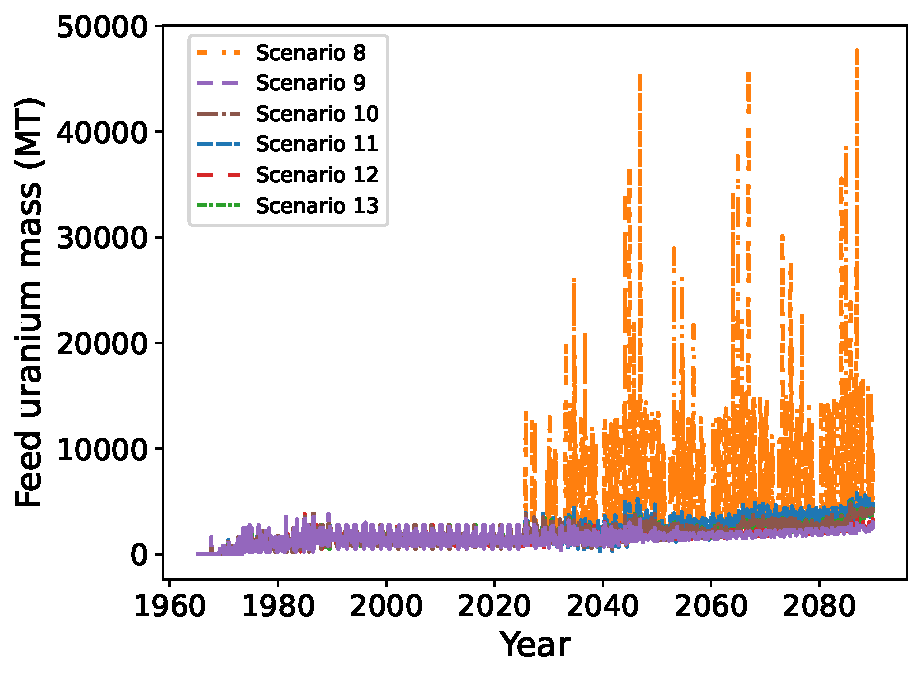
\includegraphics[width=\textwidth]{1percent_feed.pdf}
        \caption{Mass of feed uranium to produce enriched uranium sent to 
        all reactors between 1965-2090.}
        \label{fig:1percent_all_feed}
    \end{subfigure}
    \hfill
    \begin{subfigure}[b]{0.45\textwidth}
        \centering
        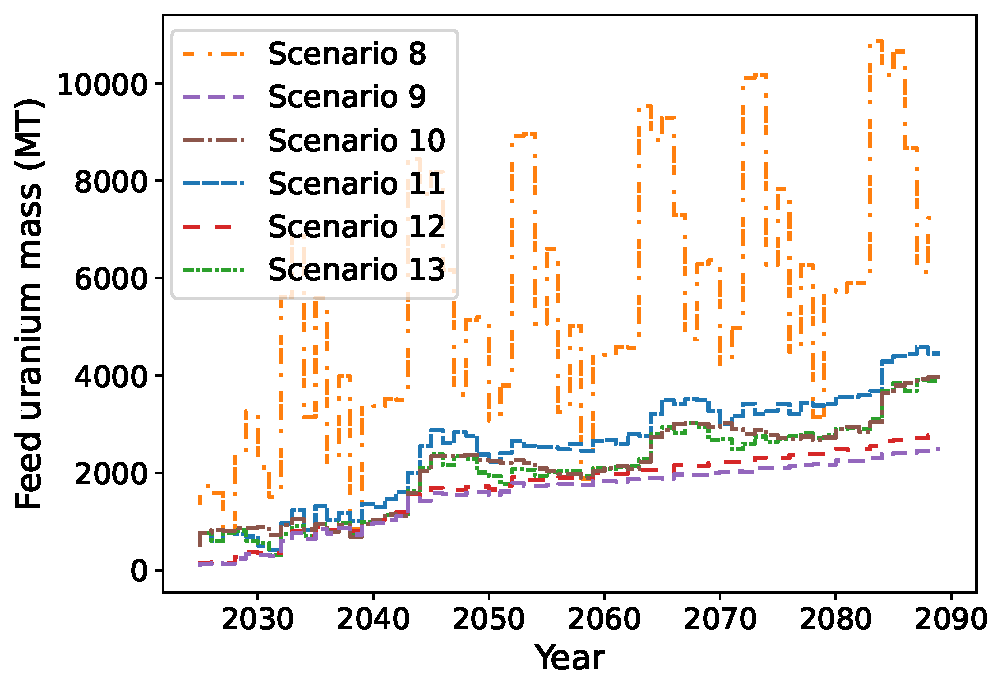
\includegraphics[width=\textwidth]{1percent_AR_feed.pdf}
        \caption{Annual average mass of feed uranium to produce enriched 
        uranium sent to advanced reactors between 2025-2090.}
        \label{fig:1percent_AR_feed}
    \end{subfigure}
    \begin{subfigure}[b]{0.45\textwidth}
        \centering
        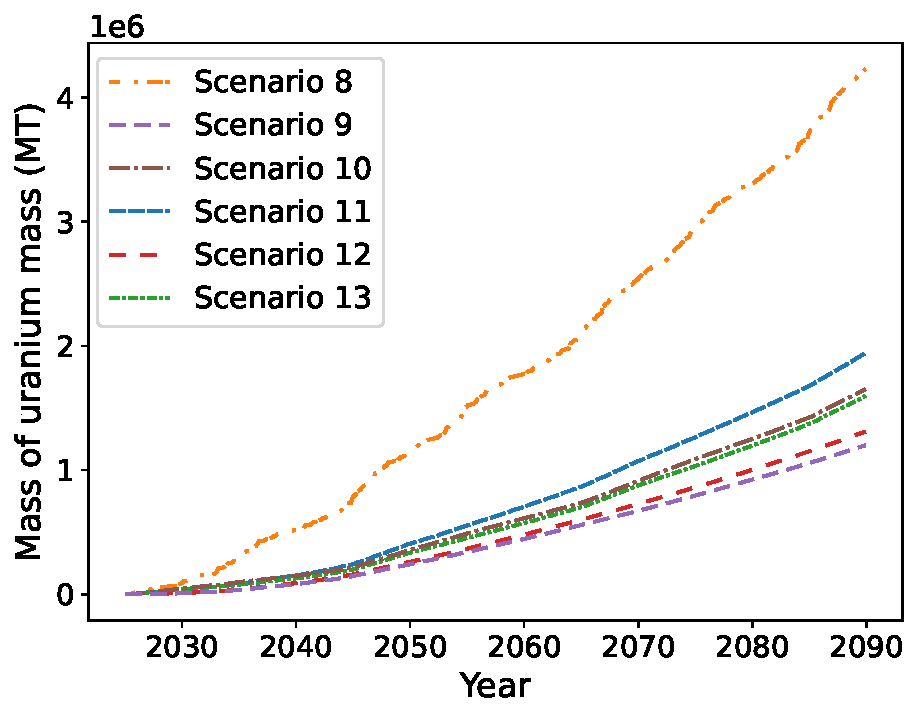
\includegraphics[width=\textwidth]{1percent_feed_cumulative.pdf}
        \caption{Cumulative mass of feed uranium to produce enriched uranium sent to 
        advanced reactors between 2025-2090.}
        \label{fig:1percent_feed_cumulative}
    \end{subfigure}
       \caption{Mass of feed uranium required to produce enriched uranium
       at each time step in Scenarios 8-13.}
       \label{fig:1percent_feed}
\end{figure}

\begin{table}
    \centering 
    \caption{Metrics for feed uranium required by advanced reactors 
    between 2025-2090 in Scenarios 8-13.}
    \label{tab:1percent_feed}
    \begin{tabular}{c c c c c}
        \hline
        Scenario & Average (t/month) & \gls{HALEU} Average  
        (t/month) & Maximum (t) & Cumulative (t)\\\hline
        8 & 5,503 & 5,503 & 41,931 & 4,287,011\\
        9 & 1,486 & 1,486 & 2,944 & 1,158,116\\
        10 & 1,758 & 1,758 & 3,446 & 1,369,598\\
        11 & 2,080 & 356.3 & 5,058 & 1,620,993\\
        12 & 1,592 & 1,062 & 3,166 & 1,240,700\\
        13 & 1,737 & 1,696 & 3,483 & 1,353,701\\
        \hline
    \end{tabular}
\end{table}

The maximum feed uranium required varies between 2.0-7.6 times the monthly 
average of all feed uranium, which is similar to the ratios of the 
maximum and average masses required for enriched uranium. Scenario 8 
requires the largest maximum peak of 
feed uranium, corresponding to the deployment of 823 \glspl{MMR}. Because 
of 
the large number of reactors and the large mass of feed uranium required 
in Scenario 8, the cumulative mass of feed uranium quickly diverges from 
the cumulative mass of the other scenarios after the transition start time. 

\section{SWU capacity}
\subsection{No growth scenarios}
The \gls{SWU} capacity required to produce the enriched uranium for 
the no growth scenarios follows a similar pattern as 
the feed uranium required by each scenario (Figure \ref{fig:nogrowth_swu}, 
Table \ref{tab:nogrowth_swu}). Scenario 2 requires the largest monthly 
average capacity, average capacity to produce \gls{HALEU}, and maximum 
capacity needed. Scenario 6 requires the smallest average for the total 
\gls{SWU} capacity, which differs from the feed material requirements, 
and Scenario 5 requires the smallest average 
\gls{SWU} capacity to produce \gls{HALEU}. Scenario 6 requires the least 
\gls{SWU} capacity because it primarily deploys Xe-100s, which require the 
smallest \gls{SWU} capacity to produce a core-load of fuel. However, it 
also deploys VOYGRs, which require the lowest product assay to decrease the 
\gls{SWU} capacity required. 
Scenario 2 requires a larger average \gls{SWU} capacity 
than the \glspl{LWR} before 2025 and Scenario 4 requires the same average 
\gls{SWU} capacity as the \glspl{LWR} before 2025. 

\begin{figure}
    \centering
    \begin{subfigure}[b]{0.45\textwidth}
        \centering
        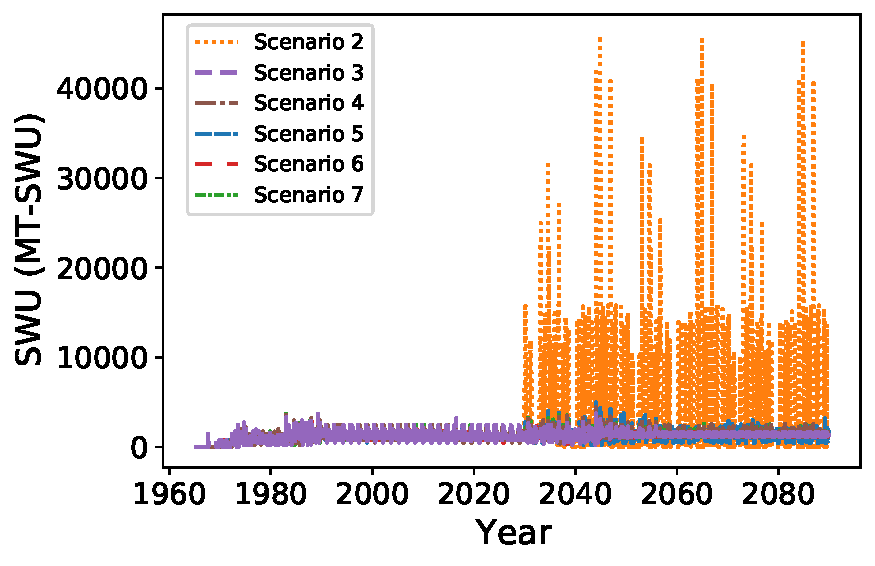
\includegraphics[width=\textwidth]{nogrowth_SWU.pdf}
        \caption{Monthly \gls{SWU} capacity required to enrich the  
        uranium sent to all reactors between 1965-2090.}
        \label{fig:nogrowth_all_SWU}
    \end{subfigure}
    \hfill
    \begin{subfigure}[b]{0.45\textwidth}
        \centering
        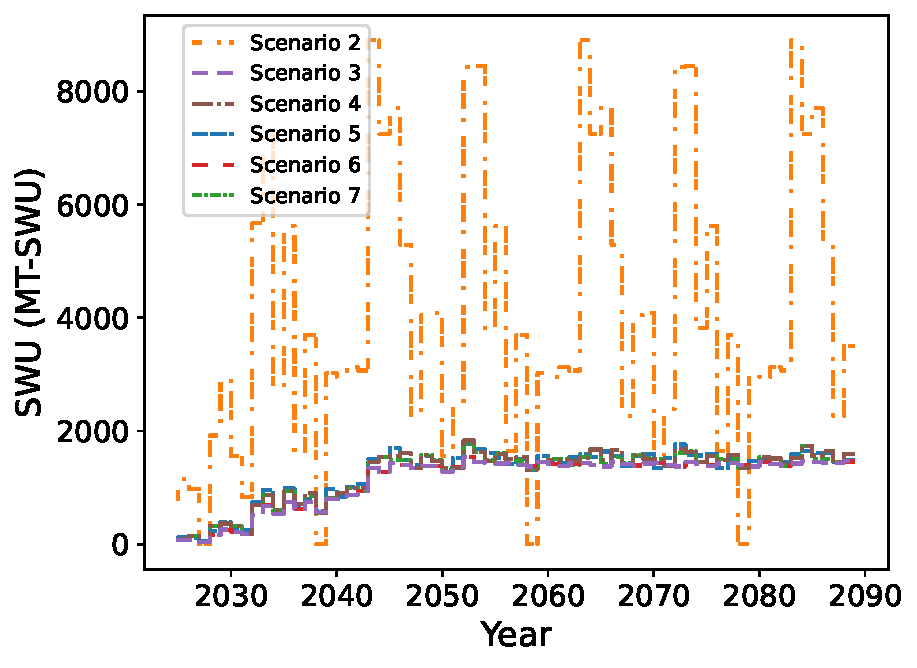
\includegraphics[width=\textwidth]{nogrowth_AR_SWU.pdf}
        \caption{Annual average \gls{SWU} capacity required to enrich 
        the uranium sent to advanced reactors between 2025-2090.}
        \label{fig:nogrowth_AR_SWU}
    \end{subfigure}
       \caption{\gls{SWU} capacity required to produce enriched uranium 
       for reactors in Scenarios 2-7.}
       \label{fig:nogrowth_swu}
\end{figure}

\begin{table}
    \centering 
    \caption{Metrics for \gls{SWU} capacity to enrich uranium for 
    advanced reactors between 2025-2090 in Scenarios 2-7.}
    \label{tab:nogrowth_swu}
    \begin{tabular}{c c c c}
        \hline
        Scenario & Average  (MT-SWU/month) & Average
        for \gls{HALEU} (MT-SWU/month) & Maximum (MT-SWU)\\\hline
        2 & 4,010 & 4,010 & 45,424 \\
        3 & 1,090 & 1,090 & 2,991\\
        4 & 1,192 & 1,192 & 3,668\\
        5 & 1,145 & 138.5 & 4,228 \\
        6 & 1,087 & 1,017 & 3,050\\
        7 & 1,167 & 1,161 & 3,735\\
        \hline
    \end{tabular}
\end{table}

The \gls{SWU} capacity required to produce \gls{HALEU} decreases when 
deploying the VOYGR along with the other reactors, with the exception 
of deploying the VOYGR with both \gls{HALEU}-fueled reactors, as noted 
with the feed uranium requirements. 
Scenario 5 requires the least \gls{SWU} capacity to produce 
\gls{HALEU} because most of the enriched uranium in this 
scenario is for VOYGRs which don't require \gls{HALEU}. This 
scenario demonstrates how a decrease in the product assay decreases 
the \gls{SWU} requirements despite an increase in the product mass. 

The maximum \gls{SWU} capacity required to meet enriched uranium demand 
varies between 2.7-11.3 times the monthly average for all \gls{SWU}. 
The magnitude differences between the average and the maximum pose potential 
problems for facility design and nonproliferation safeguards. Facilities 
will likely need to be built at a capacity greater than the average 
monthly requirement in order to produce enough enriched uranium to meet 
the peak demands. However, such a design may result in idle enrichment 
capacity during time periods in which the additional capacity is 
not needed to meet peaks, which poses a proliferation risk. 

\subsection{1\% growth scenarios}
The \gls{SWU} capacity required to meet the enriched uranium demand of 
the 1\% growth scenarios 
follows the same patterns as the \gls{SWU} capacity required in the no 
growth scenarios (Figure \ref{fig:1percent_swu}, Table \ref{tab:1percent_swu}).
Scenario 8 requires the largest average \gls{SWU} 
capacity and the largest \gls{SWU} capacity to create \gls{HALEU}. 
Scenario 12 requires the smallest average \gls{SWU} capacity for all 
advanced reactors and Scenario 11 requires the smallest \gls{SWU} capacity 
to create \gls{HALEU}. Comparing 
the average capacity and the average capacity to produce \gls{HALEU} 
shows that most or all of the \gls{SWU} capacity needed is to produce 
\gls{HALEU}, except in Scenario 11. The 
maximum \gls{SWU} capacity required ranges between 2.1-7.4 times 
the average \gls{SWU} capacity required by each scenario. All of these 
scenarios require more \gls{SWU} capacity than the \glspl{LWR} before 
2025. 

\begin{figure}
    \centering
    \begin{subfigure}[b]{0.45\textwidth}
        \centering
        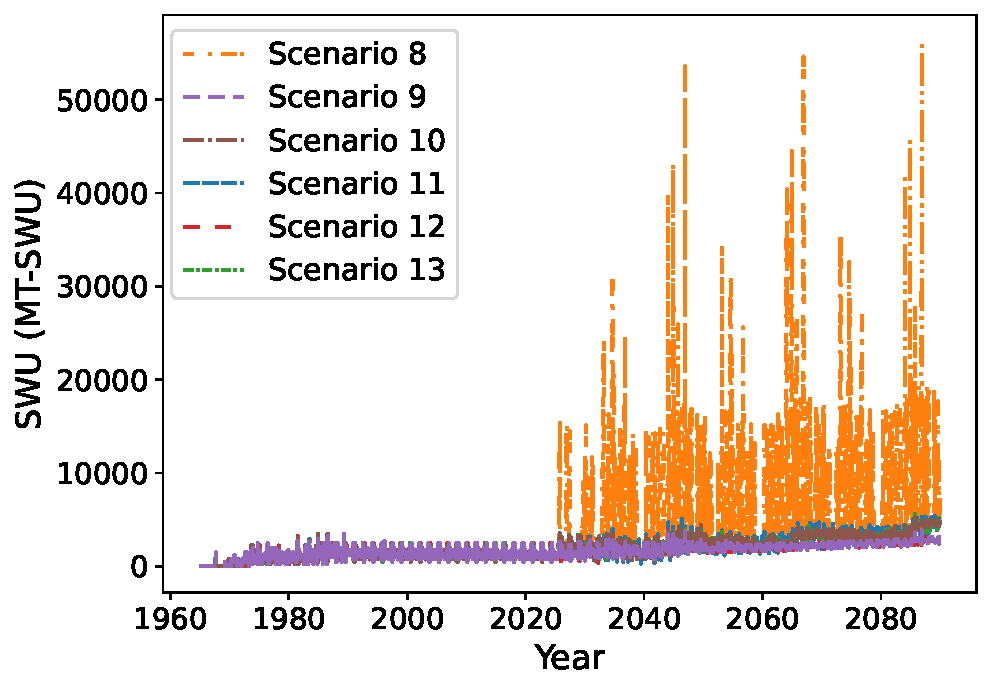
\includegraphics[width=\textwidth]{1percent_SWU.pdf}
        \caption{\gls{SWU} capacity required to enrich the mass of 
        uranium sent to all reactors between 1965-2090.}
        \label{fig:1percent_all_SWU}
    \end{subfigure}
    \hfill
    \begin{subfigure}[b]{0.45\textwidth}
        \centering
        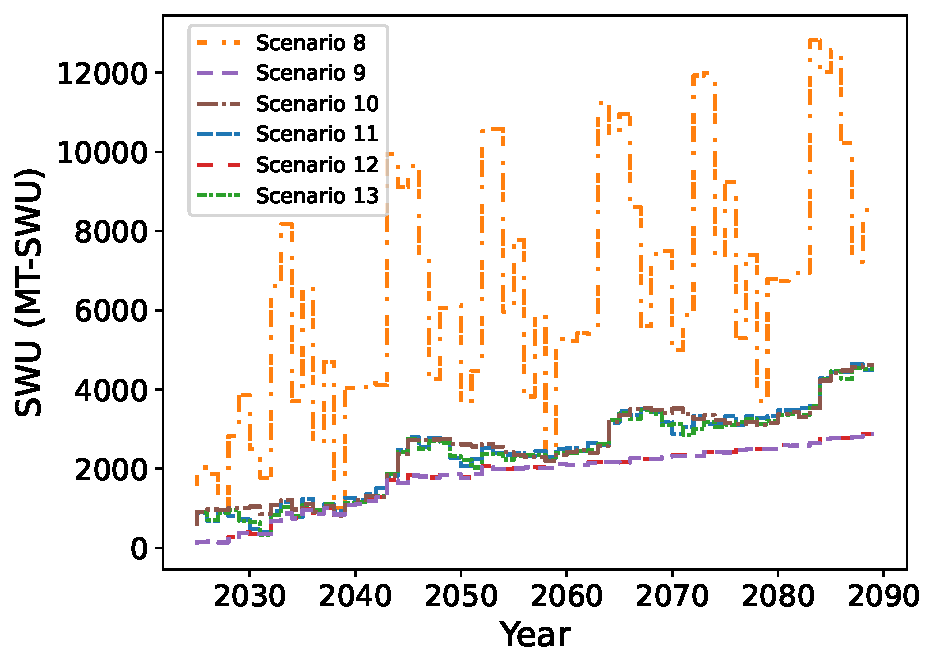
\includegraphics[width=\textwidth]{1percent_AR_SWU.pdf}
        \caption{\gls{SWU} capacity required to enrich the mass of 
        uranium sent to advanced reactors between 2025-2090.}
        \label{fig:1percent_AR_SWU}
    \end{subfigure}
       \caption{\gls{SWU} capacity required to produce enriched uranium 
       for reactors in Scenarios 8-13.}
       \label{fig:1percent_swu}
\end{figure}

\begin{table}
    \centering 
    \caption{Metrics for \gls{SWU} capacity to enrich uranium for 
    advanced reactors between 2025-2090 in Scenarios 8-13.}
    \label{tab:1percent_swu}
    \begin{tabular}{c c c c}
        \hline
        Scenario & Average (t-SWU/month) & Average  
        for \gls{HALEU} (t-SWU/month) & Maximum (t-SWU)\\\hline
        8 & 6,489 & 6,489 & 49,450 \\
        9 & 1,711 & 1,711 & 3,390 \\
        10 & 2,034 & 2,034 & 3,987\\
        11 & 1,949 & 420.2 & 4,618 \\
        12 & 1,693 & 1,223 & 3,391\\
        13 & 1,999 & 1,962 & 4,024\\
        \hline
    \end{tabular}
\end{table}

\section{Waste}
The final metric of interest for the once-through transition scenarios is 
the amount of \gls{SNF} that must be disposed of, referred to as waste 
for the purposes of this work. 
The amount of waste produced in a \gls{NFC} has implications on the options 
to treat and store the waste. A once-through fuel cycle will dispose of 
all of the 
waste discharged from the reactors, although 
the timing is affected by the duration in wet storage. The waste masses 
reported here are the masses discharged from the reactors, which 
matches the capacity needs for disposal in a dry storage system or a 
geologic repository, but not necessarily the timing of the disposal.
The masses 
presented here are the masses of all materials in the \gls{SNF}, not just 
the uranium discharged, because all materials in the \gls{SNF} must be 
disposed of. 

\subsection{No growth scenarios}
The magnitude of discharged \gls{SNF} from the advanced reactors 
(Figure \ref{fig:nogrowth_waste}) follows the same pattern as the enriched 
uranium masses, but with delayed timing. This pattern matches expectations, 
but the values are different from the masses of enriched uranium. 
This difference arises for two reasons:first, the 
\gls{SNF} masses include any carbon or oxygen in the fuel forms (UCO and 
UO$_2$), which 
are not included in the enriched uranium masses; second, the 
fuel in the reactors at the end of the simulation are not included in these 
calculations because they are not traded to the cooling pool facility.
Scenario 5 experiences the largest average mass of \gls{SNF} 
discharged but the smallest average mass of \gls{HALEU} discharged. 
Scenario 3 discharges the smallest average and cumulative mass of \gls{SNF}.
These trends are consistent with the mass of enriched uranium required 
in each scenario and the design characteristics of the advanced 
reactors deployed in each scenario. For example, Scenario 5 discharges the 
largest average mass of \gls{SNF} because it primarily deploys VOYGRs, which 
have a lower specific power than the Xe-100 and require more fuel per unit 
power than the Xe-100 and \gls{MMR}. 
The average mass of \gls{SNF} discharged by advanced reactors is less than 
the average discharged by \glspl{LWR} before 2025. 

\begin{figure}
    \centering
    \begin{subfigure}[b]{0.45\textwidth}
        \centering
        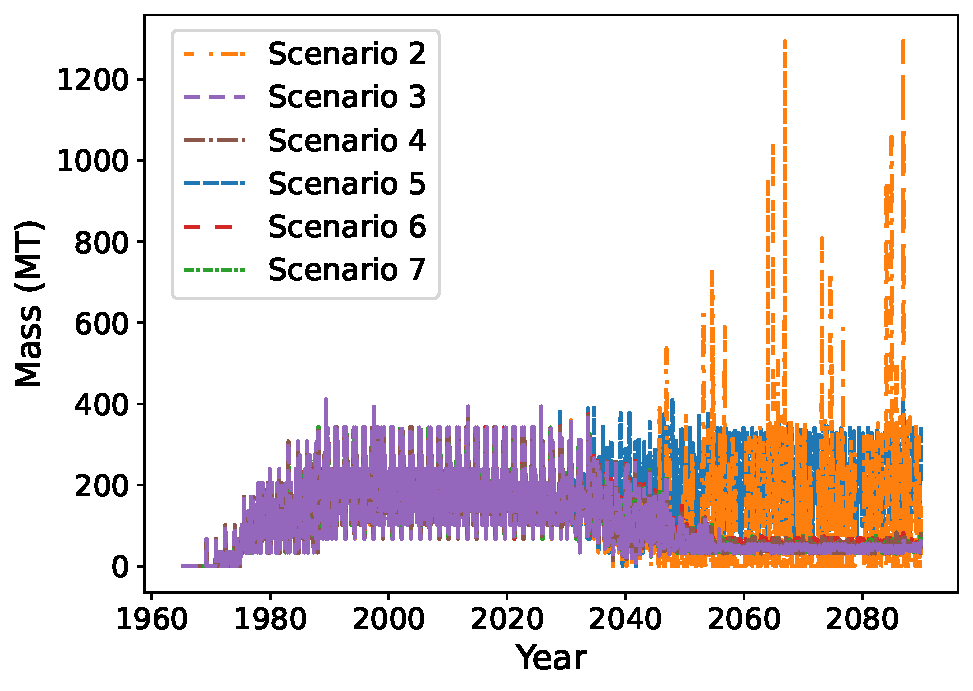
\includegraphics[width=\textwidth]{nogrowth_waste.pdf}
        \caption{Monthly mass of fuel discharged from all reactors 
        between 1965-2090.}
        \label{fig:nogrowth_all_waste}
    \end{subfigure}
    \hfill
    \begin{subfigure}[b]{0.45\textwidth}
        \centering
        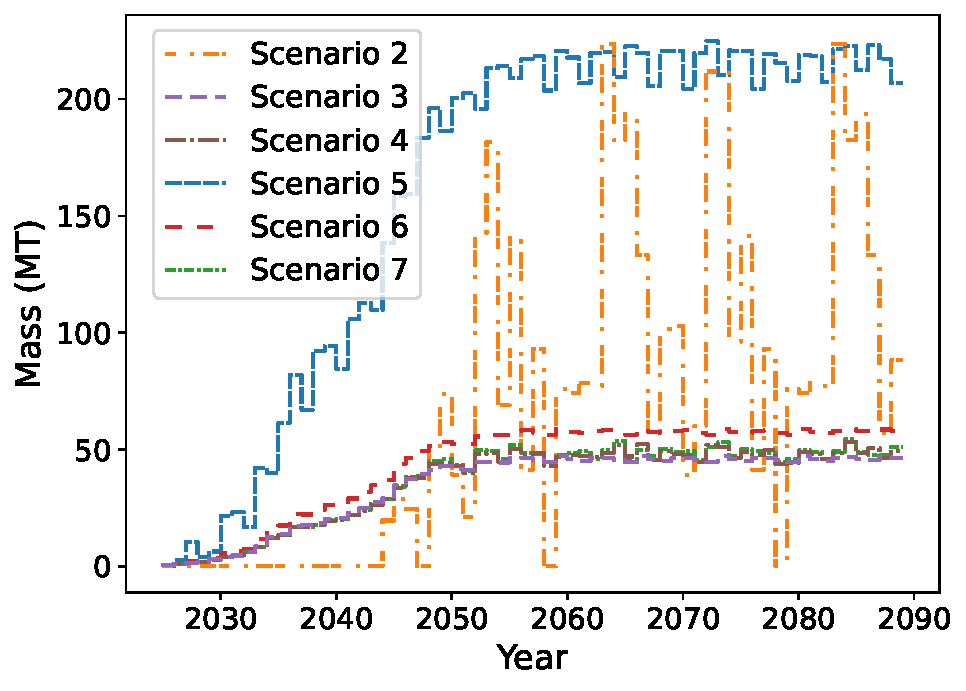
\includegraphics[width=\textwidth]{nogrowth_AR_waste.pdf}
        \caption{Annual average mass of fuel discharged from 
        advanced reactors between 2025-2090.}
        \label{fig:nogrowth_AR_waste}
    \end{subfigure}
    \begin{subfigure}[b]{0.45\textwidth}
        \centering
        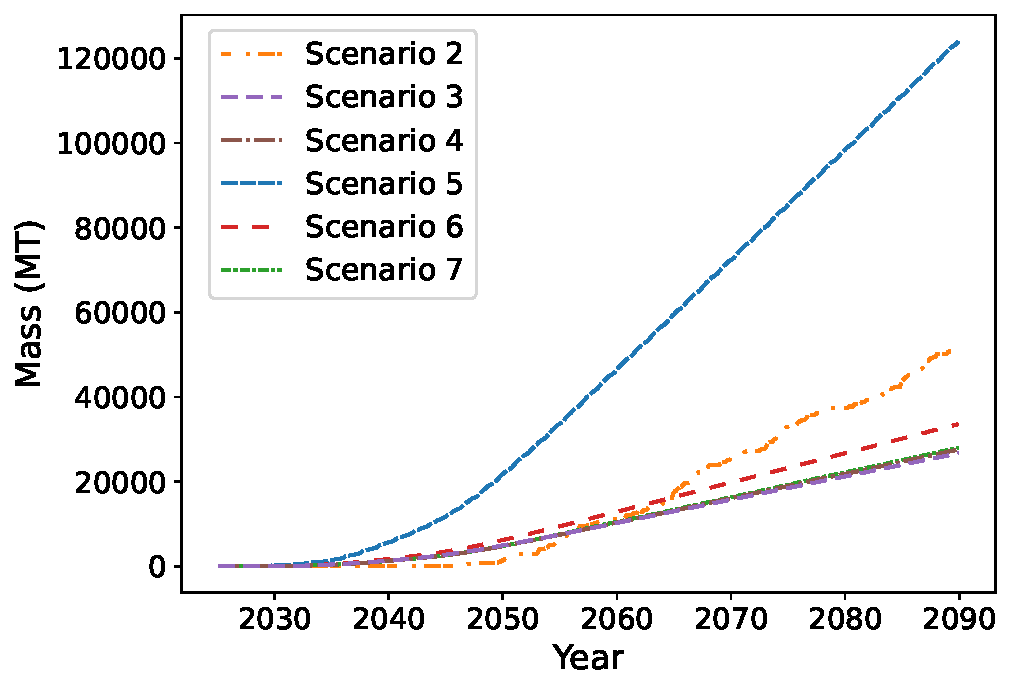
\includegraphics[width=\textwidth]{nogrowth_waste_cumulative.pdf}
        \caption{Cumulative mass of fuel discharged from advanced reactors 
        between 2025-2090.}
        \label{fig:nogrowth_waste_cumulative}
    \end{subfigure}
       \caption{Mass of fuel discharged from reactors 
       as a function of time for Scenarios 2-7. }
       \label{fig:nogrowth_waste}
\end{figure}

\begin{table}
    \centering 
    \caption{Metrics for waste discharged from advanced reactors 
    between 2025-2090 in Scenarios 2-7.}
    \label{tab:nogrowth_waste}
    \begin{tabular}{c c c c c}
        \hline
        Scenario & Average (MT/month) & Average of \gls{HALEU} 
        (MT/month) & Maximum (MT) & Cumulative (MT)\\\hline
        2 & 66.15 & 66.15 & 1,142 & 51,531\\
        3 & 32.93 & 32.93 & 55.29 & 25,654\\
        4 & 34.07 & 34.07 & 77.55 & 26,543\\
        5 & 144.9 & 2.294 & 377.0 & 112,913\\
        6 & 40.68 & 30.72 & 75.12 & 31,691\\
        7 & 34.46 & 33.62 & 83.14 & 26,848\\
        \hline
    \end{tabular}
\end{table}

The first \gls{SNF} discharged from advanced reactors is in June 
2030 for Scenarios 3, 4, 6, and 7, June 2031 
in Scenario 5, and 
December 2049 in Scenario 2. The differences in timing of first \gls{SNF} 
discharge from advanced reactors is a result of the refueling scheme of 
each type of reactor. Xe-100s, deployed in Scenarios 3, 4, 6, 
and 7, utilize online refueling and discharge \gls{SNF} 
every 6 months, results in the first discharge soon after their initial 
deployment. VOYGRs, deployed in Scenarios 4, 5, 6, and 7, have an 
18-month refueling cycle, so the first \gls{SNF} discharge for these 
reactors occurs 18 months after deployment. \glspl{MMR}, deployed in 
Scenarios 2, 4, 5, and 7, do not undergo refueling, so the first \gls{SNF} 
discharge occurs 20 years after first deployment. The shortest refueling 
time of the reactors deployed in a scenario governs when 
first \gls{SNF} discharge in that scenario. Thus, the Xe-100 is the 
governing reactor for 
Scenarios 3, 4, 6, and 7 the VOYGR is the governing reactor for Scenario  
5, and the \gls{MMR} is the governing reactor for Scenario 2 with regards 
to \gls{SNF} discharge times. 

The 
advanced reactors in all of the scenarios discharge 
less \gls{SNF} than the \glspl{LWR}. The 1982 Nuclear Waste Policy Act
\cite{noauthor_nuclear_1983} requires an initial 
repository in the US to have a capacity of 70,000 MTHM. Based on this 
capacity,  a geologic repository could store 
all of the waste produced from advanced reactors except for Scenario 5. 
To store all of the waste from advanced reactors in Scenario 5, either 
the repository capacity would need to be expanded or a second repository 
must be sited.

\subsection{1\% growth scenarios}
For the 1\% growth scenarios, similar patterns are observed to the 
no growth scenarios; Scenario 11 discharges  
the largest average mass of \gls{SNF} while also discharging
the smallest average mass of \gls{HALEU} \gls{SNF}, as shown by  
Figure \ref{fig:1percent_waste} and Table \ref{tab:1percent_waste}. 
Scenario 9 discharges the smallest average mass of \gls{SNF}. The 
first \gls{SNF} discharge 
is in November 2027 in Scenarios 9, 10, 12, and 13, in 
November 2028 in Scenario 11, and May 2047 in Scenario 8. These initial 
disposal dates are consistent with the shortest cycle time of the 
reactors deployed in each scenario (20 years in Scenario 8, 18 months in 
Scenario 11, and 6 month in Scenarios 9, 10, 12, and 13) and an 
initial deployment in May 2027. 

\begin{figure}
    \centering
    \begin{subfigure}[b]{0.45\textwidth}
        \centering
        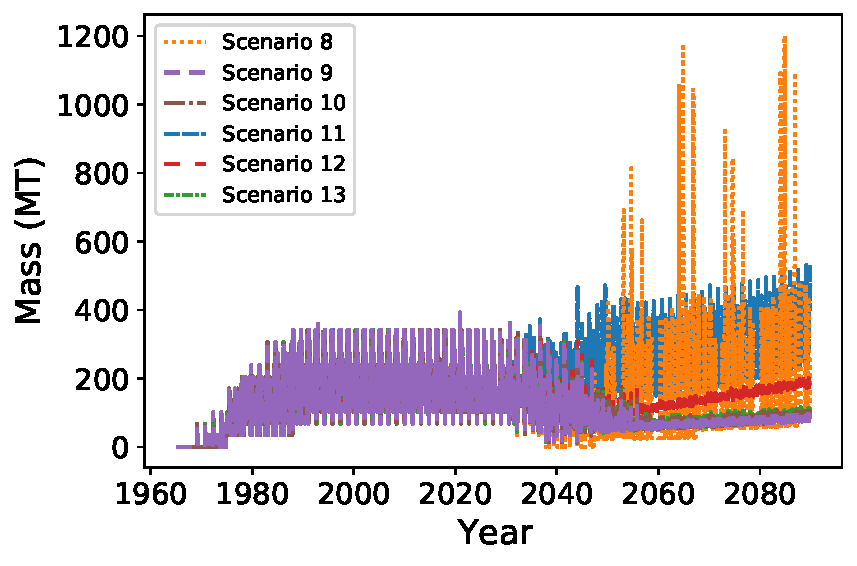
\includegraphics[width=\textwidth]{1percent_waste.pdf}
        \caption{Mass of fuel discharged from all reactors between 
        1965-2090.}
        \label{fig:1percent_all_waste}
    \end{subfigure}
    \hfill
    \begin{subfigure}[b]{0.45\textwidth}
        \centering
        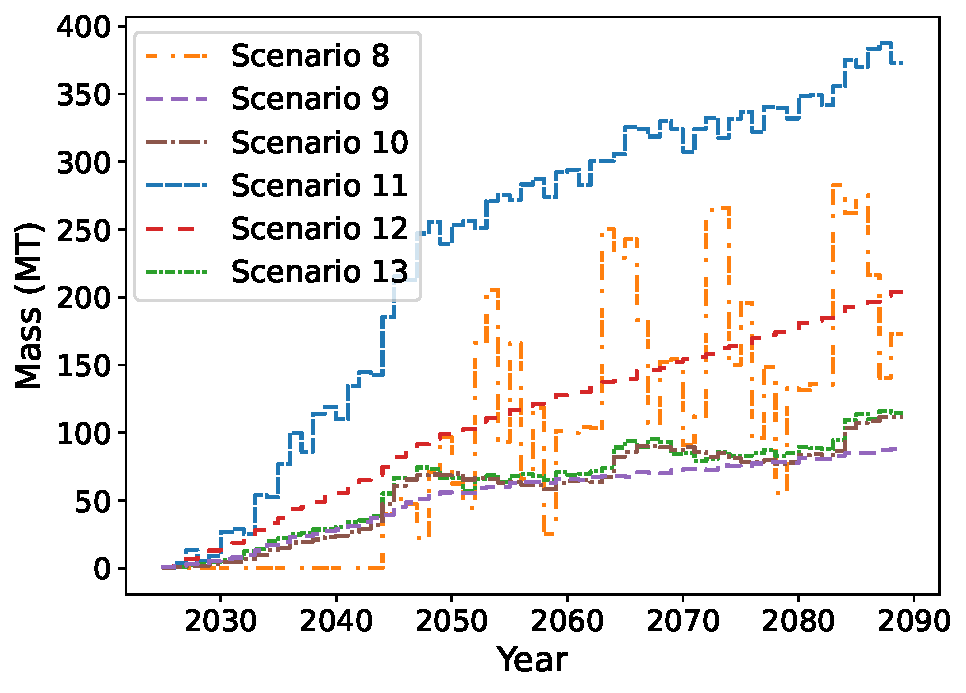
\includegraphics[width=\textwidth]{1percent_AR_waste.pdf}
        \caption{Mass of fuel discharged from advanced reactors 
        between 2025-2090.}
        \label{fig:1percent_AR_waste}
    \end{subfigure}
    \begin{subfigure}[b]{0.45\textwidth}
        \centering
        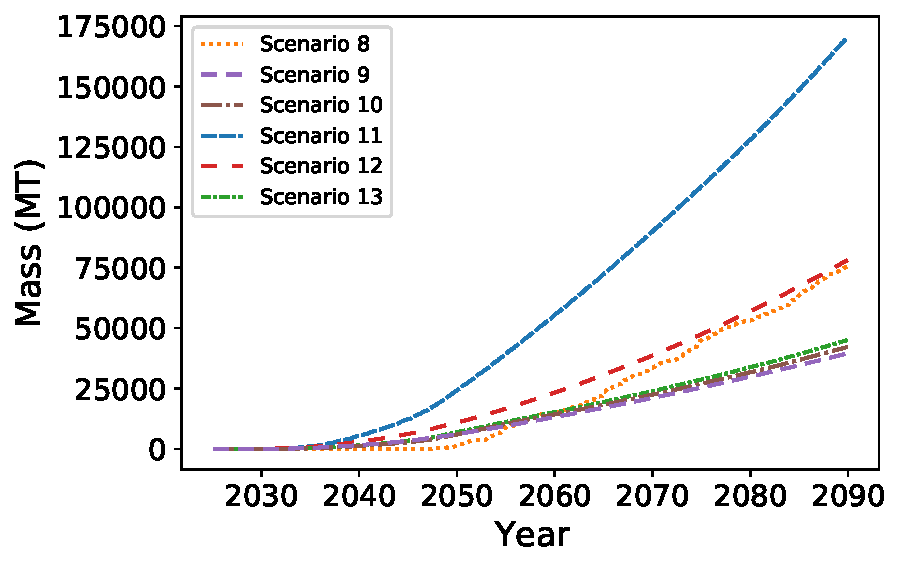
\includegraphics[width=\textwidth]{1percent_waste_cumulative.pdf}
        \caption{Cumulative mass of fuel discharged from advanced reactors 
        between 2025-2090.}
        \label{fig:1percent_waste_cumulative}
    \end{subfigure}
       \caption{Mass of fuel discharged from reactors 
       as a function of time for Scenarios 8-13. }
       \label{fig:1percent_waste}
\end{figure}

\begin{table}
    \centering 
    \caption{Metrics for waste discharged from advanced reactors 
    between 2025-2090 in Scenarios 8-13.}
    \label{tab:1percent_waste}
    \begin{tabular}{c c c c c}
        \hline
        Scenario & Average (t/month) & Average of \gls{HALEU} (t/month) 
        & Maximum (t) & Cumulative (t)\\\hline
        8 & 97.00 & 97.00 & 1,202 & 75,563 \\
        9 & 50.83 & 50.83 & 101.2 & 39,593 \\
        10 & 54.19 & 54.19 & 111.3 & 42,215 \\
        11 & 218.7 & 6.982 & 534.8 & 170,391 \\
        12 & 100.3 & 36.57 & 205.7 & 78,131 \\
        13 & 57.86 & 52.73 & 116.4 & 45,076 \\
        \hline
    \end{tabular}
\end{table}

Based on the cumulative masses, the proposed 70,000 MTHM capacity of 
a geologic repository in the US would only store the \gls{SNF} 
discharged from advanced reactors in Scenarios 8, 9, 10, and 13. Additional 
repositories or an expanded capacity of the repository would be required 
to dispose of the waste from Scenarios 11 and 12. The 
cumulative waste discharged from advanced reactors is less than the 
cumulative mass discharged from the \glspl{LWR} in all scenarios except 
Scenario 11. Scenario 11 discharges more \gls{SNF} because of the large 
number of VOYGRs it deploys to meet the increasing energy demand. 

